\clearpage

\section {Results of the $\nu_{\mu}$-disappearance analysis with the Run 1+2+3+4a (6.3933$\times10^{20}$ POT) dataset}
\label{sec:results}

%--------------------------------------------------------------------------------------
% Best-fit params & pulls
%--------------------------------------------------------------------------------------

\subsection {Best-fit oscillation parameters and systematic parameter pulls}
\label{sec:results_bestfit}

A 3-flavour $\nu_{\mu}$-disappearance fit was performed on the combined 6.3933$\times$10$^{20}$ 
POT Run 1+2+3+4a dataset, using the method described in Sec.\ 4.1 of Ref.\ \cite{OurRun123DisappAnalysis3Flavour},
in which all 44 nuisance parameters considered in this work are allowed to float. 
% A similar analysis was also carried out separately on each of the 3.0100$\times$10$^{20}$ POT Run 1+2+3 and
% 3.3833$\times$10$^{20}$ POT Run 4a datasets.

This analysis found
$|\Delta m^{2}_{32}|$ = 2.463$\times$10$^{-3}$ eV$^{2}$/c$^{4}$ and
$\sin^{2}\theta_{23}$ = 0.514
to be the best-fit values for the Run 1+2+3+4a dataset
for a fit assuming the normal mass hierarchy.
A similar best-fit value was obtained from a separate fit,
assuming the inverted mass hierarchy, of
$|\Delta m^{2}_{32}|$ = 2.530$\times$10$^{-3}$ eV$^{2}$/c$^{4}$ and
$\sin^{2}\theta_{23}$ = 0.511.
% Similar best-fit values were obtained from separate fits to subsets of the full dataset. 
% The fit to the Run 1+2+3 dataset gave best-fit values of 
% $|\Delta m^{2}_{32}|$ = x.xxx$\times$10$^{-3}$ eV$^{2}$/c$^{4}$ and 
% $\sin^{2}\theta_{23}$ = x.xxx, while a fit to the Run 4a dataset gave 
% $|\Delta m^{2}_{32}|$ = x.xxx$\times$10$^{-3}$ eV$^{2}$/c$^{4}$ 
% and $\sin^{2}\theta_{23}$ = x.xxx.

The results of these fits are summarized in Tab.\ \ref{tab:data_fits:best_fit_values}. In this table are 
the best-fit oscillation parameters, the observed and expected number of single-ring $\mu$-like events,
and the values of $\chi^{2}$ per degree of freedom at the best-fit.

The pull for each systematic parameter $f$ included in the fit, is calculated as
\begin{equation}
\frac{f_{bf} - f_{nom}}{\sigma_{bf}},
\end{equation}
where 
$f_{bf}$ is the best-fit value of the systematic parameter,
$f_{nom}$ is the nominal value of the parameter (corresponding to no systematic variation), and
$\sigma_{bf}$ is the Hesse error output from Minuit.

The pulls of all 44 nuisance parameters allowed to float in the fit are shown in 
Figs.\ \ref{fig:results_data1234a_pulls:normal} and \ref{fig:results_data1234a_pulls:inverted}
for the fit to the Run 1+2+3+4a dataset assuming the normal and inverted mass hierarchy respectively.
% , and in 
% Figs.\ \ref{fig:results_data123_pulls}-\ref{fig:results_data4a_pulls} for the
% fits to the Run 1+2+3 and Run 4a datasets.
From these figures, it is apparent that most systematic parameters barely move from their nominal values.
We note that, although all 44 systematic parameters are allowed to float in the fit,
only 2(2) of them move by more than $\pm$0.1$\sigma$ for the normal(inverted) fit. 
When a systematic parameter that is free to move stays close to its nominal value, this means that 
the reduction in $\chi^{2}$ from moving that parameter is less than the corresponding increase 
in the penalty term ($\chi^{2}$ is defined in equation 3 in Sec.\ 4.1.5 in Ref.\ \cite{OurRun123DisappAnalysis3Flavour}). 
Only certain systematics are able to change the predicted reconstructed energy spectrum to a 
sufficient extent to offset the penalty term. 

%...........................................................
%
% Table summarizing best-fit results
%
\begin{table}
\centering
\begin{tabular}{| l | l | c | c | c  c | c | c |}
\hline
Analysis & Run period & $\sin^{2}\theta_{23}$ & $\Delta m_{32}^2$ & N$_{obs}$ & N$_{exp}$ & $\chi^2_{bf} / ndf$ & p-value \\
\hline
2013 3-flavour Normal   & Run 1+2+3+4a & 0.514 &  2.463 $\cdot 10^{-3}$ & 115 & 115.77 & 64.88/73 & 0.88 \\
2013 3-flavour Inverted & Run 1+2+3+4a & 0.511 &  2.530 $\cdot 10^{-3}$ & 115 & 115.72 & 64.87/73 & 0.89 \\
% 2013 3-flavour & Run 4a       & x.xxx &  x.xxx $\cdot 10^{-3}$ & xx & xx.xx & xx.xx/xx & x.xx \\
% 2013 3-flavour & Run 1+2+3    & x.xxx &  x.xxx $\cdot 10^{-3}$ & xx & xx.xx & xx.xx/xx & x.xx \\
% 2012 3-flavour & Run 1+2+3    & 1.000 &  2.443 $\cdot 10^{-3}$ & 58 & 57.97 & 56.04/71 & 0.83 \\
\hline
\end{tabular}
\caption{
  Summary of best-fit parameters for the oscillation fits to the Run 1+2+3+4a dataset. %Run 1+2+3, Run 4a, and combined Run 1+2+3+4a datasets.
  % The 2012 result is taken from the analysis presented in \cite{OurRun123DisappAnalysis3Flavour}
  The quoted best-fit $\chi^2$ values ($\chi^2_{bf}$) were computed from Eq.\ 5 in Sec.\ 4.1.5 in Ref.\ \cite{OurRun123DisappAnalysis3Flavour} 
  with the reconstructed energy binning used in each fit.
  The table also shows the p-values obtained from the goodness-of-fit test described in Sec.\ 4.2 in \cite{OurRun123DisappAnalysis3Flavour} for all fits.
}
\label{tab:data_fits:best_fit_values}
\end{table}

%...........................................................
%
% Systematic parameter pulls 
%

\begin{figure*}[htb]
\center
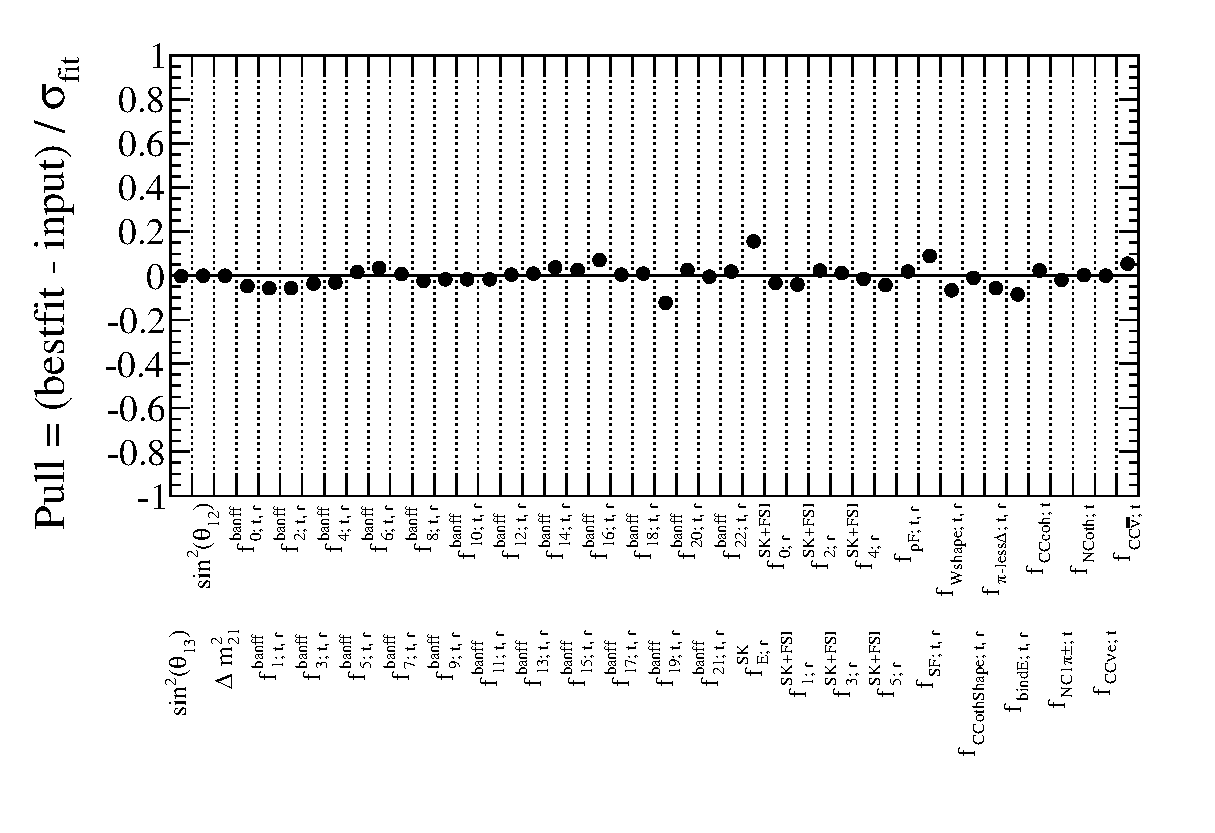
\includegraphics[width=50pc,angle=270]{./images/data_results/run1234a_normal/run1-4_nuis3fixdcp_sintheta_normal_pulls}
\caption {
  Systematic parameter pulls for the fit to the Run 1+2+3+4a dataset.
  The normal mass hierarchy is assumed.
}
\label{fig:results_data1234a_pulls:normal}
\end{figure*}

\begin{figure*}[htb]
\center
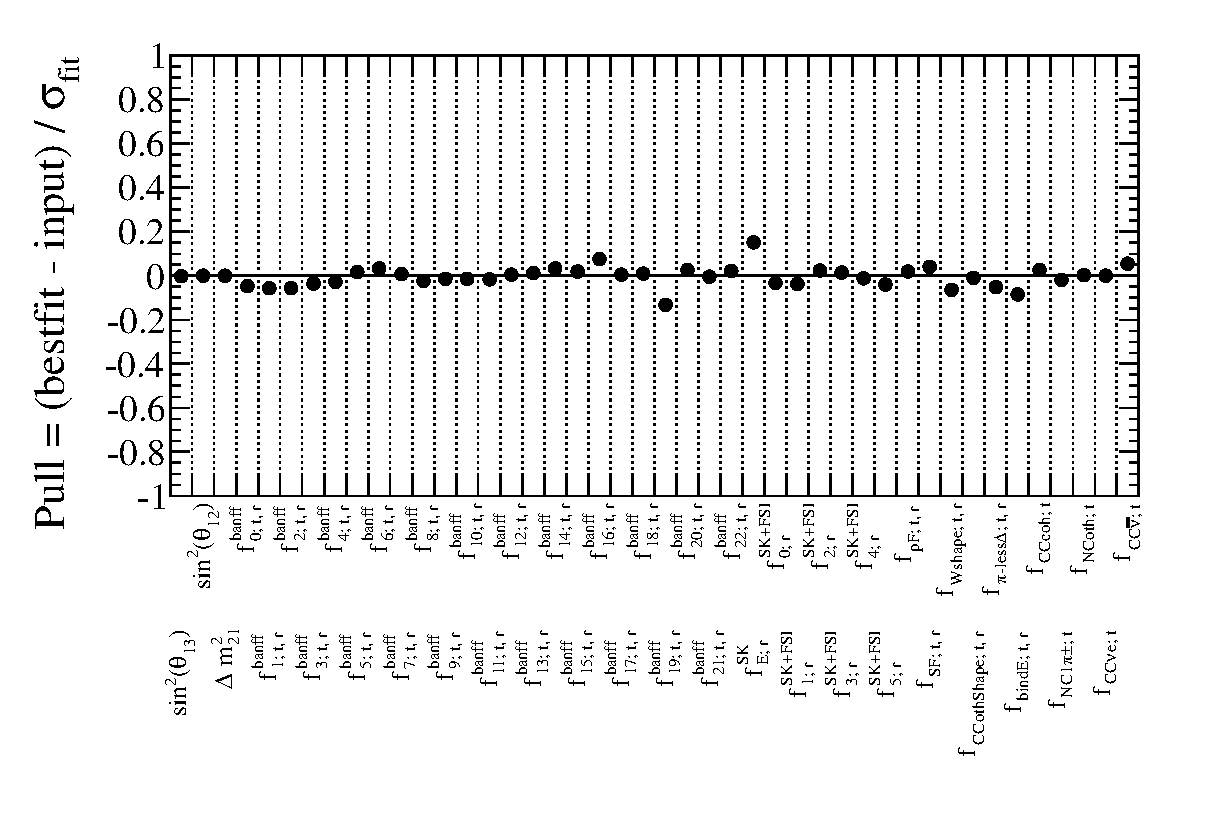
\includegraphics[width=50pc,angle=270]{./images/data_results/run1234a_inverted/run1-4_nuis3fixdcp_sintheta_inverted_pulls}
\caption {
  Systematic parameter pulls for the fit to the Run 1+2+3+4a dataset.
  The inverted mass hierarchy is assumed.
}
\label{fig:results_data1234a_pulls:inverted}
\end{figure*}

% \begin{figure*}[htb]
% \begin{minipage}[t]{0.48\linewidth}
% \center
% 
\includegraphics[width=22pc,angle=270]{./images/placeholder.eps}
% \caption {
%   Systematic parameter pulls for the fit to the Run 1+2+3 dataset.
% }
% \label{fig:results_data123_pulls}
% \end{minipage}
% \hspace{0.06\linewidth}
% \begin{minipage}[t]{0.48\linewidth}
% \center
% 
\includegraphics[width=22pc,angle=270]{./images/placeholder.eps}
% \caption {
%   Systematic parameter pulls for the fit to the Run 4a dataset.
% }
% \label{fig:results_data4a_pulls}
% \end{minipage}
% \end{figure*}

%--------------------------------------------------------------------------------------
% Goodness of fit tests
%--------------------------------------------------------------------------------------

\subsection {Goodness-of-fit tests}
\label{sec:results_gof}

Goodness-of-fit tests were performed as described in Sec.\ 4.2 of Ref. \cite{OurRun123DisappAnalysis3Flavour},
and the p-values for the fits to the Run 1+2+3+4a dataset %, Run 1+2+3 and Run 4a datasets
are shown in Tab.\ \ref{tab:data_fits:best_fit_values}. 
The $\chi^2$ distribution from which the p-value was calculated is shown for the 
Run 1+2+3+4a data in Figs.\ \ref{fig:results_data1234a_goodness:normal} and \ref{fig:results_data1234a_goodness:inverted}
for the normal and inverted mass hierarchy respectively.
Both %All
fits have a high degree of plausibility.

%..................................
%
% Chisq_{gof} distributions
%

\begin{figure*}[htb]
\center
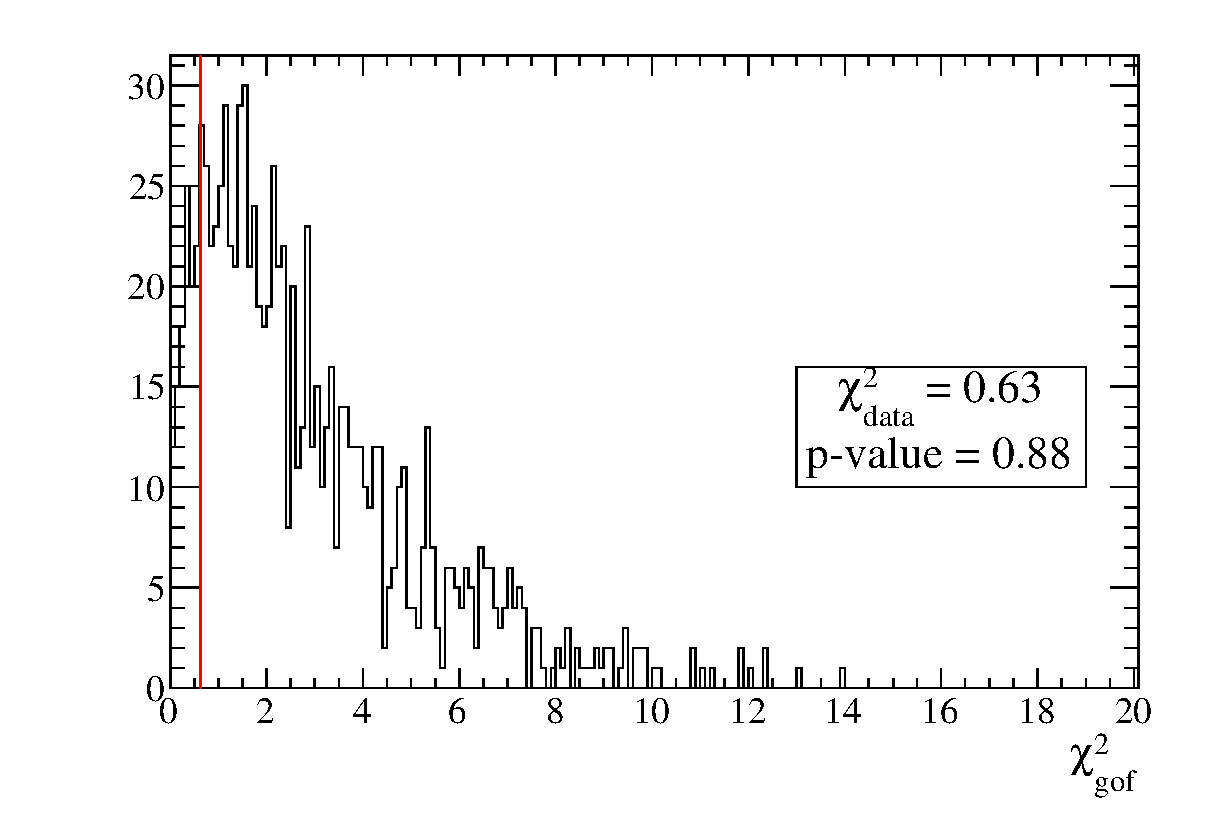
\includegraphics[width=24pc]{./images/data_results/run1234a_normal/goodness_run1-4_nuis3fixdcp_sintheta_normal}
\caption {
  Distribution of $\chi^2_{gof}$, the goodness-of-fit (gof) $\chi^2$, 
  from 1k toy MC experiments generated at the Run 1+2+3+4a best-fit oscillation point.
  The $\chi^2_{gof}$ value for the Run 1+2+3+4a data ($\chi^2_{data}$) is highlighted.
  The normal mass hierarchy is assumed.
}
\label{fig:results_data1234a_goodness:normal}
\end{figure*}

\begin{figure*}[htb]
\center
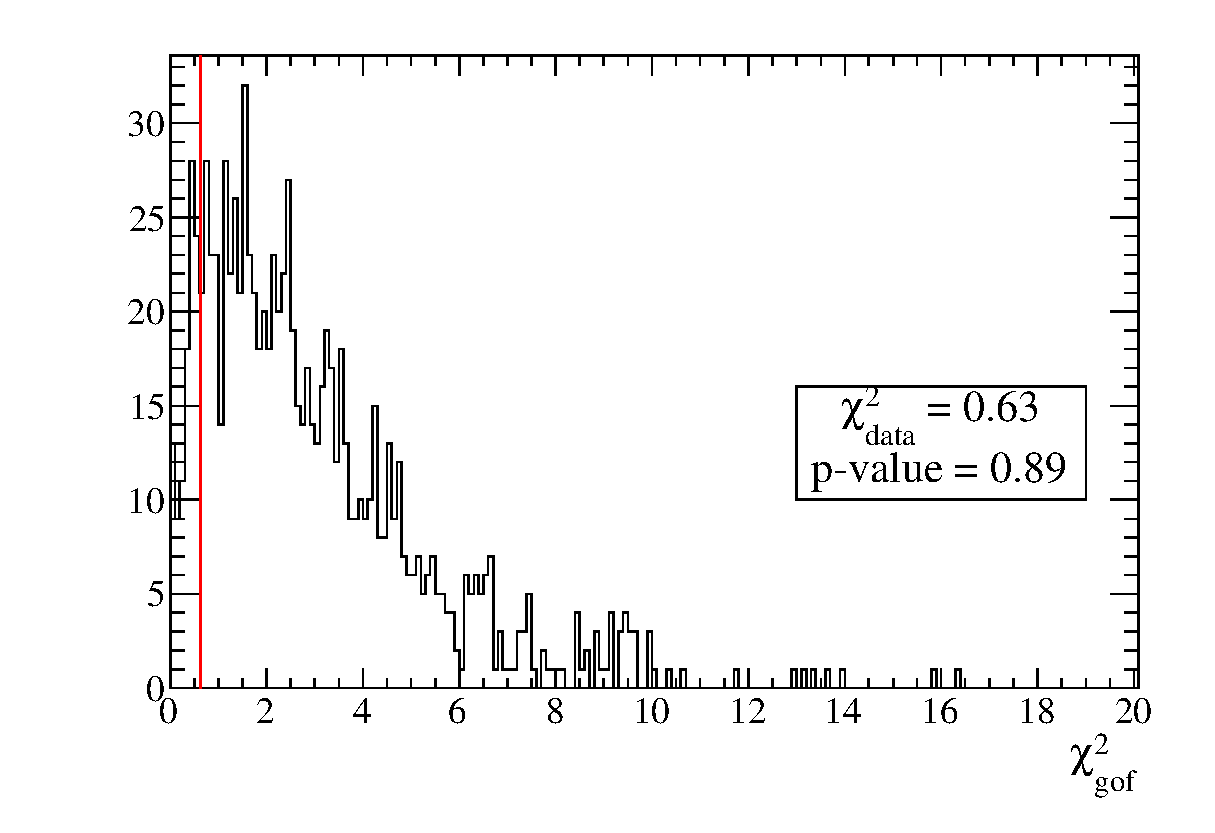
\includegraphics[width=24pc]{./images/data_results/run1234a_inverted/goodness_run1-4_nuis3fixdcp_sintheta_inverted}
\caption {
  Distribution of $\chi^2_{gof}$, the goodness-of-fit (gof) $\chi^2$, 
  from 1k toy MC experiments generated at the Run 1+2+3+4a best-fit oscillation point.
  The $\chi^2_{gof}$ value for the Run 1+2+3+4a data ($\chi^2_{data}$) is highlighted.
  The inverted mass hierarchy is assumed.
}
\label{fig:results_data1234a_goodness:inverted}
\end{figure*}


%--------------------------------------------------------------------------------------
% Best-fit spectra
%--------------------------------------------------------------------------------------

\subsection {Best-fit single-ring $\mu$-like reconstructed energy spectra}
\label{sec:results_bestfit_spectra}

The reconstructed neutrino energy distribution of the single-ring $\mu$-like events in the Run 1+2+3+4a dataset assuming the normal mass hierarchy
is shown in Fig.\  \ref{fig:results_data1234a_spectrum:normal} along with the best-fit prediction and the prediction made 
under the no-oscillation hypothesis. Also shown is the ratio between the data and the no-oscillation spectrum and 
the ratio between the best-fit spectrum and the the no-oscillation spectrum; in both of these ratios, the characteristic 
energy-dependent deficit can be clearly seen.
The corresponding spectra for the fit assuming the inverted mass hierarchy is shown in Fig.\ \ref{fig:results_data1234a_spectrum:inverted}.
% The equivalent spectra for the Run 1+2+3 and Run 4a datasets are also shown in 
% Figs.\ \ref{fig:results_data123_spectrum} and \ref{fig:results_data4a_spectrum} respectively. 
All these distributions are shown in the 73-bin scheme in reconstructed 
neutrino energy that was used in the fitting procedure (see Sec.\ 2.2.5 in Ref.\ \cite{OurRun123DisappAnalysis3Flavour}).

Since the reconstructed energy binning used in the fit is relatively fine, it can be beneficial to see the above distributions using 
a coarser binning. The best-fit spectra obtained from the fits to the Run 1+2+3+4a %, Run 1+2+3 and Run 4a datasets are
dataset is 
shown using a coarser binning scheme\footnote{
  16 reconstructed energy bins arranged as follows:
  1 0.3-GeV bin from 0 - 0.3 GeV,
  8 0.1-GeV bins from 0.3 - 1.1 GeV,
  1 0.15-GeV bin from 1.1 GeV - 1.25 GeV,
  1 0.25-GeV bin from 1.25 - 1.5 GeV GeV,
  1 0.5-GeV bin from 1.5 - 2 GeV,
  2 1-GeV bin from 2-4 GeV,
  1 2-GeV bin from 4-6 GeV and
  1 bin above 6 GeV.
} 
in Figs.\
\ref{fig:results_data1234a_spectrum_coarse:normal} and \ref{fig:results_data1234a_spectrum_coarse:inverted}
for the normal and inverted mass hierarchy respectively.
% \ref{fig:results_data1234_spectrum_coarse} and
% \ref{fig:results_data4a_spectrum_coarse}
% respectively. 
It is also interesting to see the 32 components of the best-fit spectrum, each of which is calculated separately 
in this analysis. These components are shown for the Run 1+2+3+4a fit in 
Figs.\  \ref{fig:results_data1234a_spectrum_components:normal} and \ref{fig:results_data1234a_spectrum_components:inverted}
for the normal and inverted mass hierarchy respectively.
In these plots, the components of the spectrum are grouped into 5 categories: 
$\nu_{\mu}$ CCQE, $\nu_{\mu}$ CCnonQE, $\bar{\nu}_{\mu}$ CC, $\nu_{e}$/$\bar{\nu}_{e}$ CC and NC.

\label{fig:results_data1234a_spectrum_comparison_coarse}
Finally, the normal and inverted mass hierarchy best-fit predictions are compared for the Run 1+2+3+4a dataset only in
Fig.\ \ref{fig:results_data1234a_spectrum_comparison},
using the 73 reconstructed energy bins used in the fit, and in
Fig. \ref{fig:results_data1234a_spectrum_comparison_coarse},
using the coarser binning described above.
The two best-fit spectra are nearly identical.

% {\color{red} Another comparison we could show in Run 1+2+3, Run 4a and Run 1+2+3+4a best-fit predictions,
% all scaled to  Run 1+2+3+4a exposure. We could also show a comparison between the 5 components listed above 
% and, also, show results of a test to check consistency between the 3 best-fit predictions}.

%...........................................................
%
% Best-fit spectra and ratios (73 bins)
%
\begin{figure*}[htb]
  \begin{minipage}[t]{0.8\linewidth}
    \center
    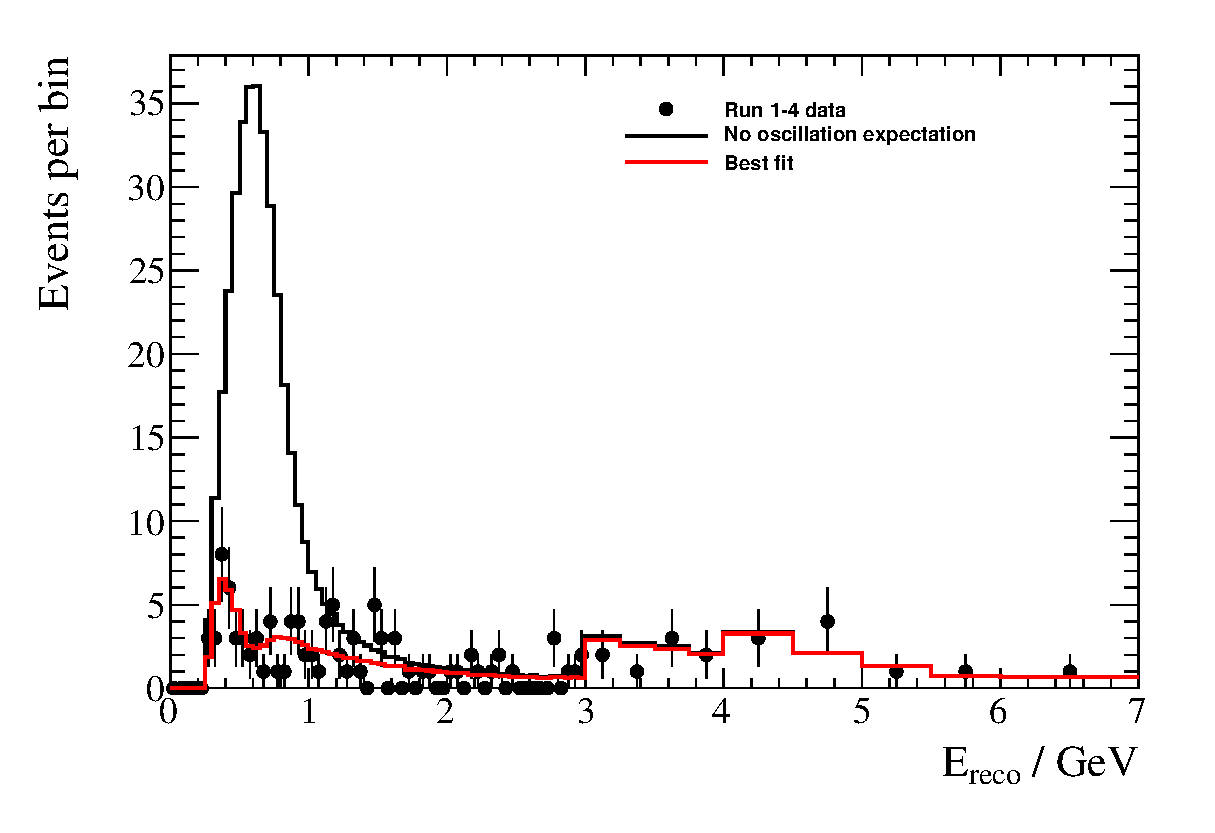
\includegraphics[width=28pc]{./images/data_results/run1234a_normal/run1-4_nuis3fixdcp_sintheta_normal_spectrum}
  \end{minipage}
  \vfill
  \begin{minipage}[t]{0.8\linewidth}
    \center
    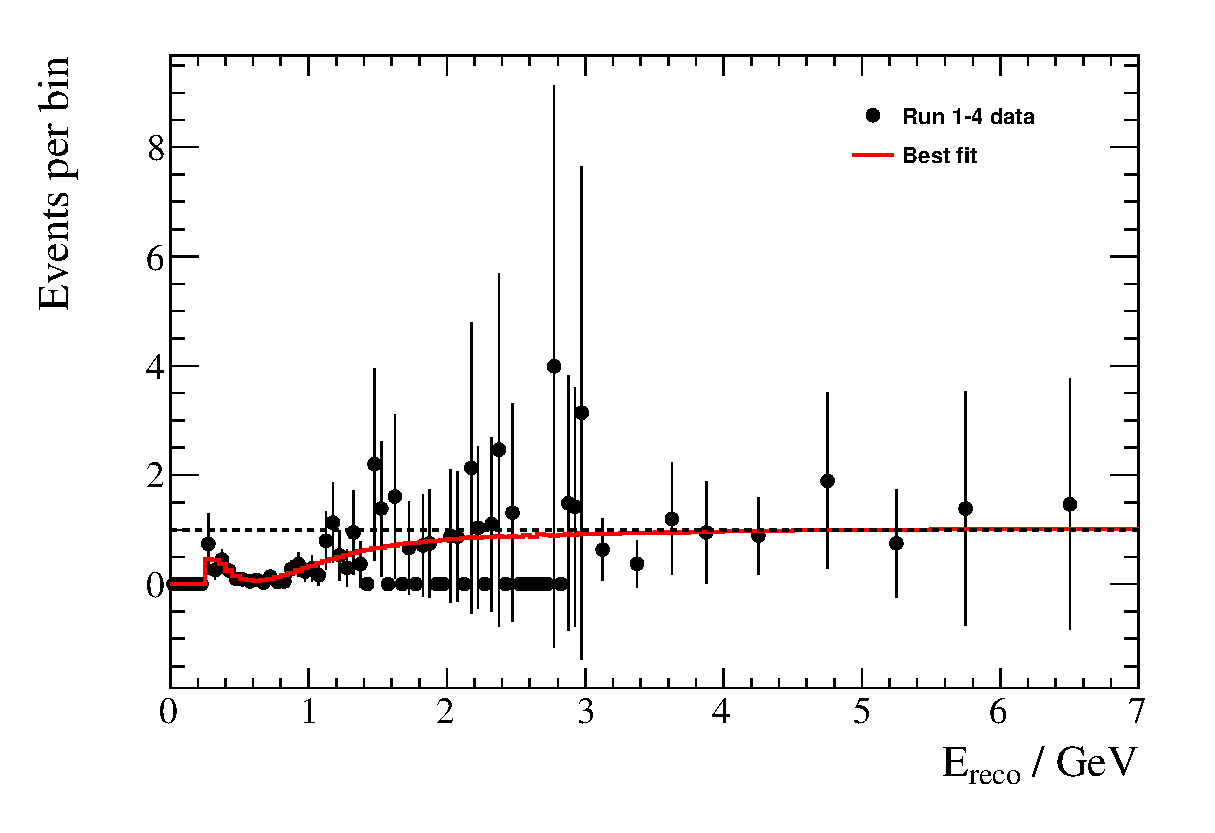
\includegraphics[width=28pc]{./images/data_results/run1234a_normal/run1-4_nuis3fixdcp_sintheta_normal_spectrum_ratio}
  \end{minipage}
  \caption {
    Best-fit reconstructed energy spectrum (top) obtained from the fit to the combined Run 1+2+3+4a dataset.
    The Run 1+2+3+4a dataset and the prediction obtained from the no-oscillation hypothesis are also shown.
    The spectra are shown using the 73 bins used in the fit (see Sec.\ 2.2.5 in Ref.\ \cite{OurRun123DisappAnalysis3Flavour}).
    The ratio of the data and best-fit distribution to the no-oscillation hypothesis is shown 
    in the bottom plot. The characteristic energy-dependent deficit can be clearly seen.
    The normal mass hierarchy is assumed.
  \label{fig:results_data1234a_spectrum:normal}
  }
\end{figure*}

\begin{figure*}[htb]
  \begin{minipage}[t]{0.8\linewidth}
    \center
    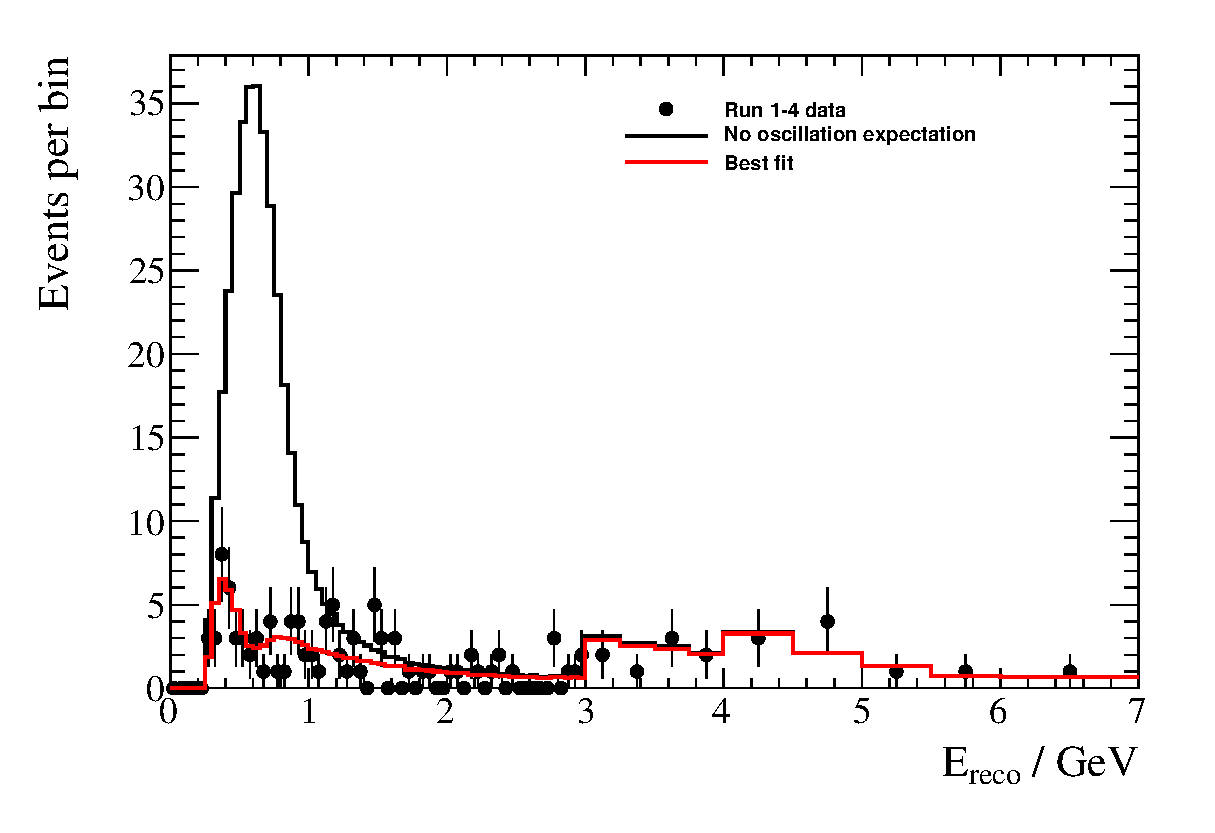
\includegraphics[width=28pc]{./images/data_results/run1234a_inverted/run1-4_nuis3fixdcp_sintheta_inverted_spectrum}
  \end{minipage}
  \vfill
  \begin{minipage}[t]{0.8\linewidth}
    \center
    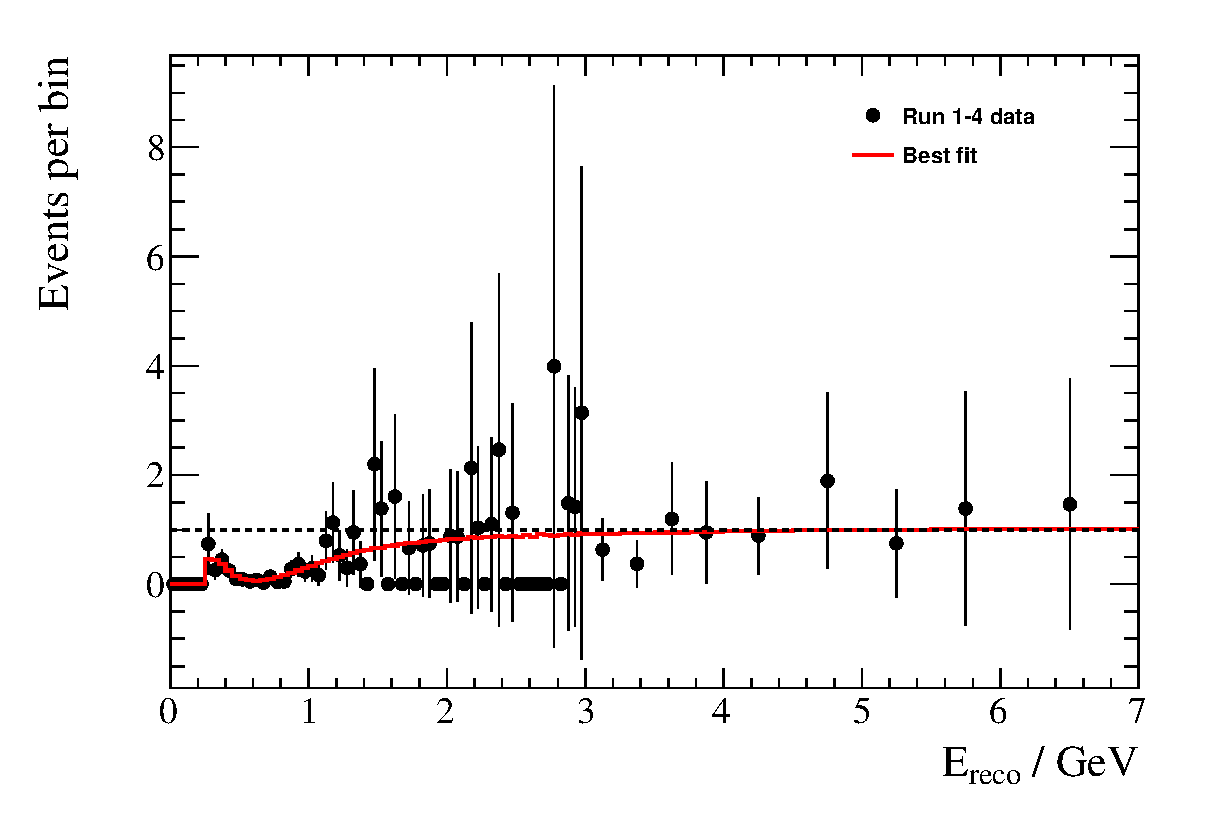
\includegraphics[width=28pc]{./images/data_results/run1234a_inverted/run1-4_nuis3fixdcp_sintheta_inverted_spectrum_ratio}
  \end{minipage}
  \caption {
    Best-fit reconstructed energy spectrum (top) obtained from the fit to the combined Run 1+2+3+4a dataset.
    The Run 1+2+3+4a dataset and the prediction obtained from the no-oscillation hypothesis are also shown.
    The spectra are shown using the 73 bins used in the fit (see Sec.\ 2.2.5 in Ref.\ \cite{OurRun123DisappAnalysis3Flavour}).
    The ratio of the data and best-fit distribution to the no-oscillation hypothesis is shown 
    in the bottom plot. The characteristic energy-dependent deficit can be clearly seen.
    The inverted mass hierarchy is assumed.
  \label{fig:results_data1234a_spectrum:inverted}
  }
\end{figure*}

% \begin{figure*}[htb]
% \begin{minipage}[t]{0.48\linewidth}
% \center
% 
\includegraphics[width=20pc]{./images/placeholder.eps}
% \caption {
%   As in Fig.\ \ref{fig:results_data1234a_spectrum}, but for the Run 1+2+3 dataset only.
% }
% \label{fig:results_data123_spectrum}
% \end{minipage}
% \hspace{0.06\linewidth}
% \begin{minipage}[t]{0.48\linewidth}
% \center
% 
\includegraphics[width=20pc]{./images/placeholder.eps}
% \caption {
%   As in Fig.\ \ref{fig:results_data1234a_spectrum}, but for the Run 4a dataset only.
% }
% \label{fig:results_data4a_spectrum}
% \end{minipage}
% \end{figure*}

%...........................................................
%
% Best-fit spectra and ratios (coarse binning)
%
\begin{figure*}[htb]
  \begin{minipage}[t]{0.8\linewidth}
    \center
    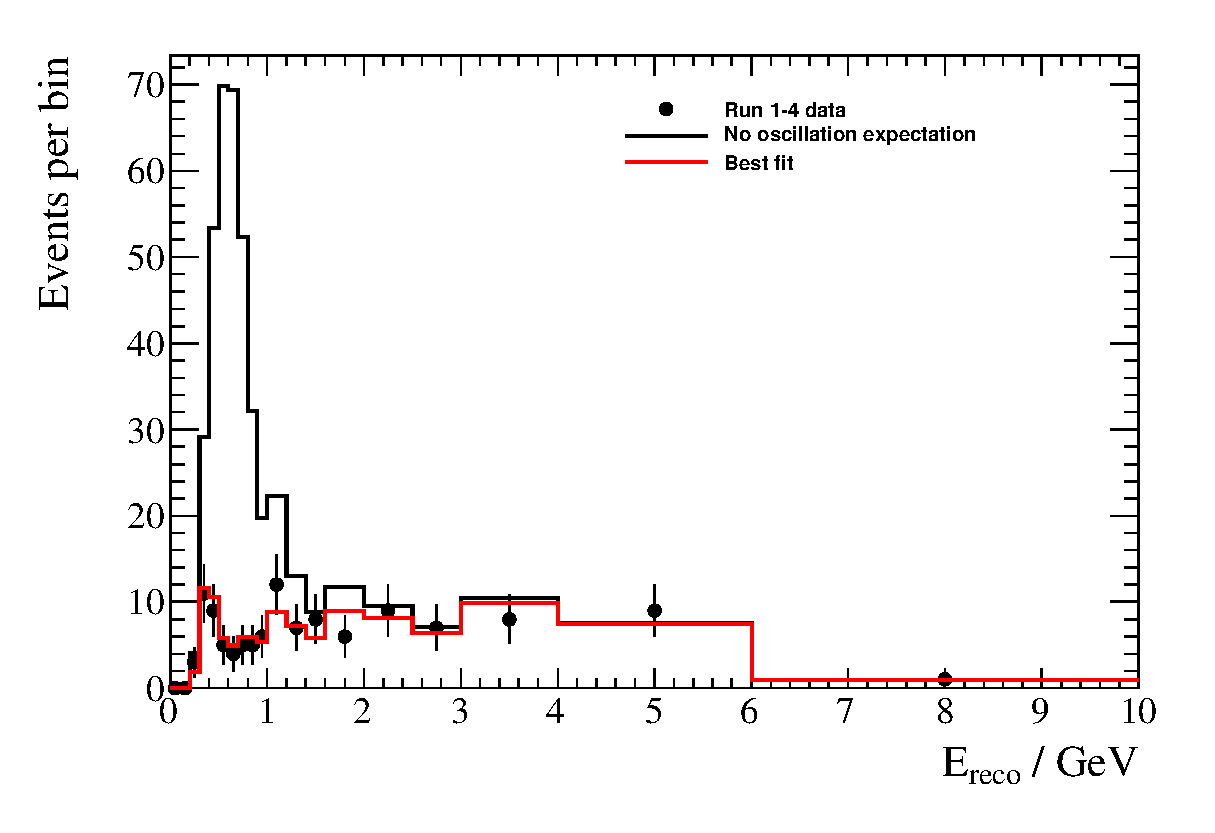
\includegraphics[width=28pc]{./images/data_results/run1234a_normal/run1-4_nuis3fixdcp_sintheta_normal_spectrum_rebin}
  \end{minipage}
  \vfill
  \begin{minipage}[t]{0.8\linewidth}
    \center
    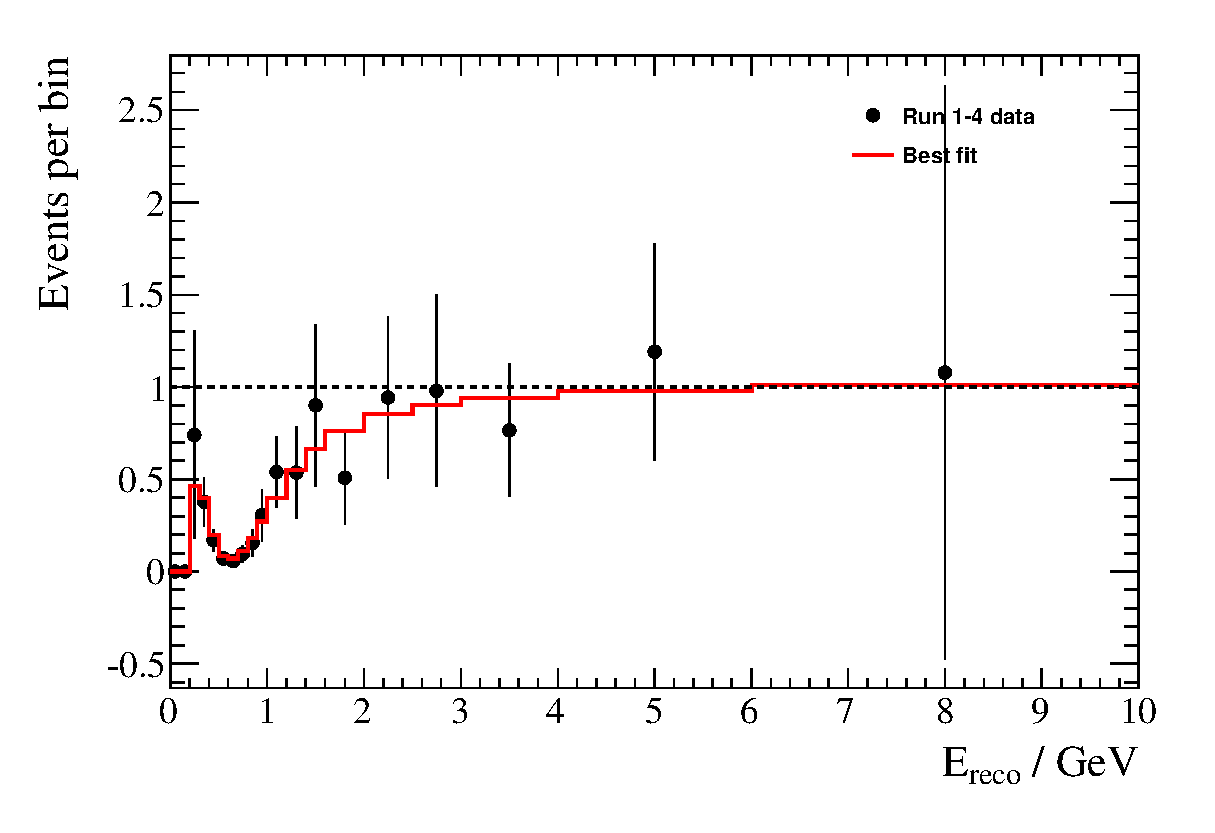
\includegraphics[width=28pc]{./images/data_results/run1234a_normal/run1-4_nuis3fixdcp_sintheta_normal_spectrum_ratio_rebin}
  \end{minipage}
  \caption {
    Best-fit reconstructed energy spectrum (top) obtained from the fit to the combined Run 1+2+3+4a dataset.
    The Run 1+2+3+4a dataset and the prediction obtained from the no-oscillation hypothesis are also shown.
    The spectra are shown using the coarse binning scheme discussed in the text (see Sec.\ \ref{sec:results_bestfit_spectra}).
    The characteristic energy-dependent deficit can be clearly seen.
    The normal mass hierarchy is assumed.
  \label{fig:results_data1234a_spectrum_coarse:normal}
  }
\end{figure*}

\begin{figure*}[htb]
  \begin{minipage}[t]{0.8\linewidth}
    \center
    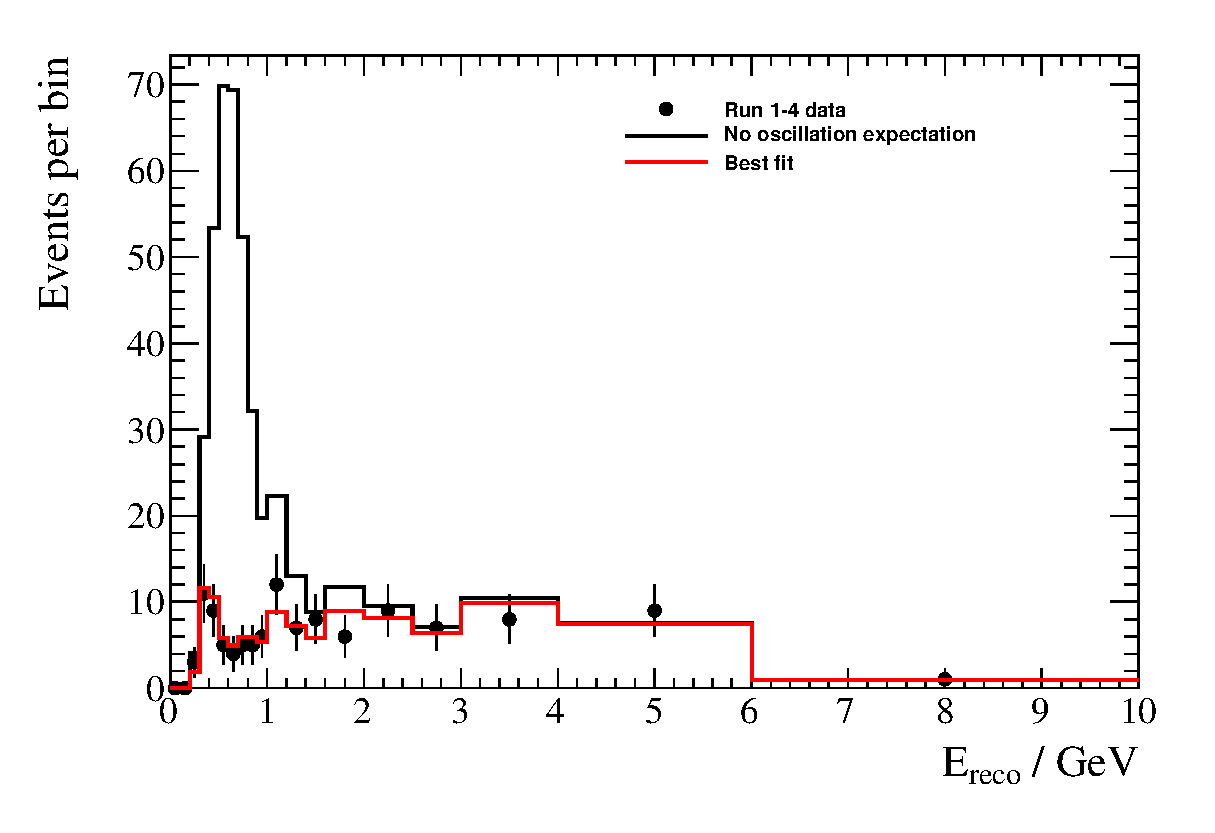
\includegraphics[width=28pc]{./images/data_results/run1234a_inverted/run1-4_nuis3fixdcp_sintheta_inverted_spectrum_rebin}
  \end{minipage}
  \vfill
  \begin{minipage}[t]{0.8\linewidth}
    \center
    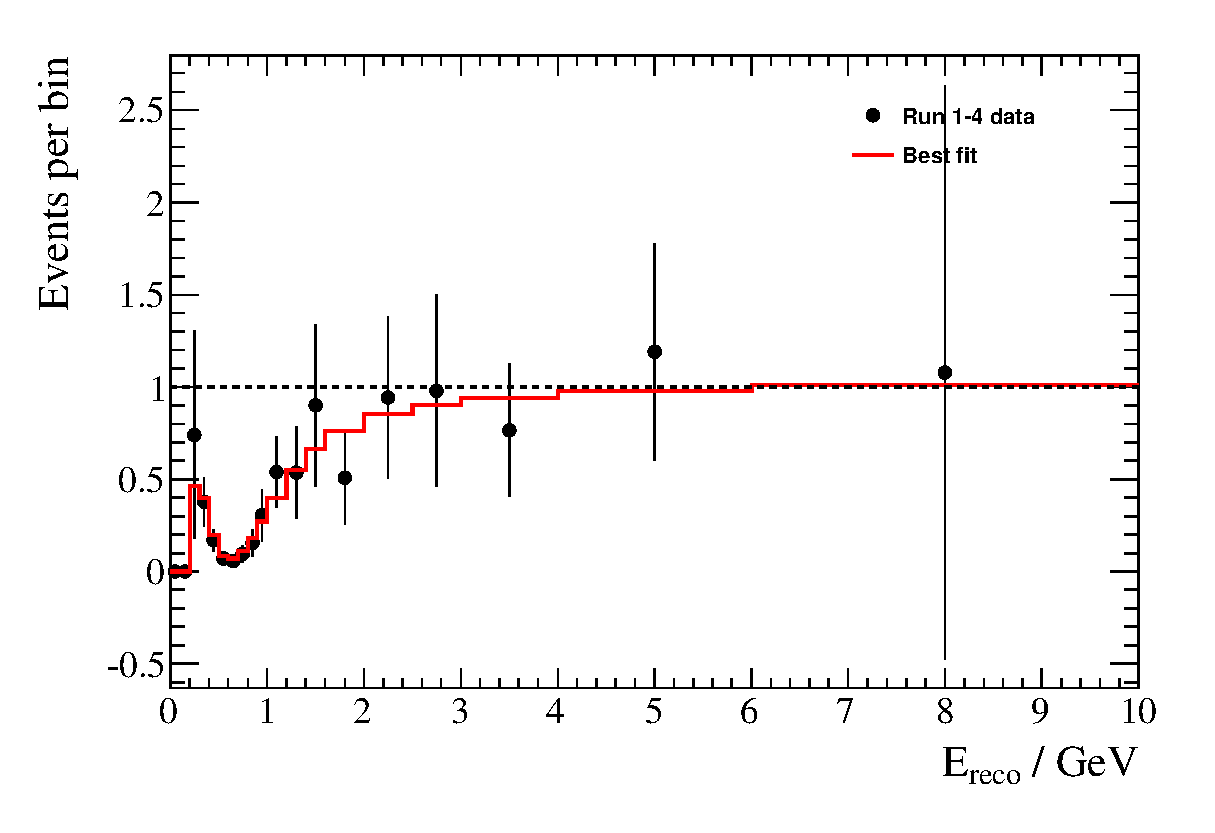
\includegraphics[width=28pc]{./images/data_results/run1234a_inverted/run1-4_nuis3fixdcp_sintheta_inverted_spectrum_ratio_rebin}
  \end{minipage}
  \caption {
    Best-fit reconstructed energy spectrum (top) obtained from the fit to the combined Run 1+2+3+4a dataset.
    The Run 1+2+3+4a dataset and the prediction obtained from the no-oscillation hypothesis are also shown.
    The spectra are shown using the coarse binning scheme discussed in the text (see Sec.\ \ref{sec:results_bestfit_spectra}).
    The characteristic energy-dependent deficit can be clearly seen.
    The inverted mass hierarchy is assumed.
    \label{fig:results_data1234a_spectrum_coarse:inverted}
  }
\end{figure*}

% \begin{figure*}[htb]
% \begin{minipage}[t]{0.48\linewidth}
% \center
% 
\includegraphics[width=20pc]{./images/placeholder.eps}
% \caption {
%   As in Fig.\ \ref{fig:results_data1234a_spectrum_coarse}, but for the Run 1+2+3 dataset only.
% }
% \label{fig:results_data123_spectrum}
% \end{minipage}
% \hspace{0.06\linewidth}
% \begin{minipage}[t]{0.48\linewidth}
% \center
% 
\includegraphics[width=20pc]{./images/placeholder.eps}
% \caption {
%   As in Fig.\ \ref{fig:results_data1234a_spectrum_coarse}, but for the Run 4a dataset only.
% }
% \label{fig:results_data4a_spectrum}
% \end{minipage}
% \end{figure*}


%...........................................................
%
% Best-fit spectra (total and components) for `2+N' fit 
% (Run1+2+3+4a only, 73 bins)
%

\begin{figure*}[htb]
  \center
  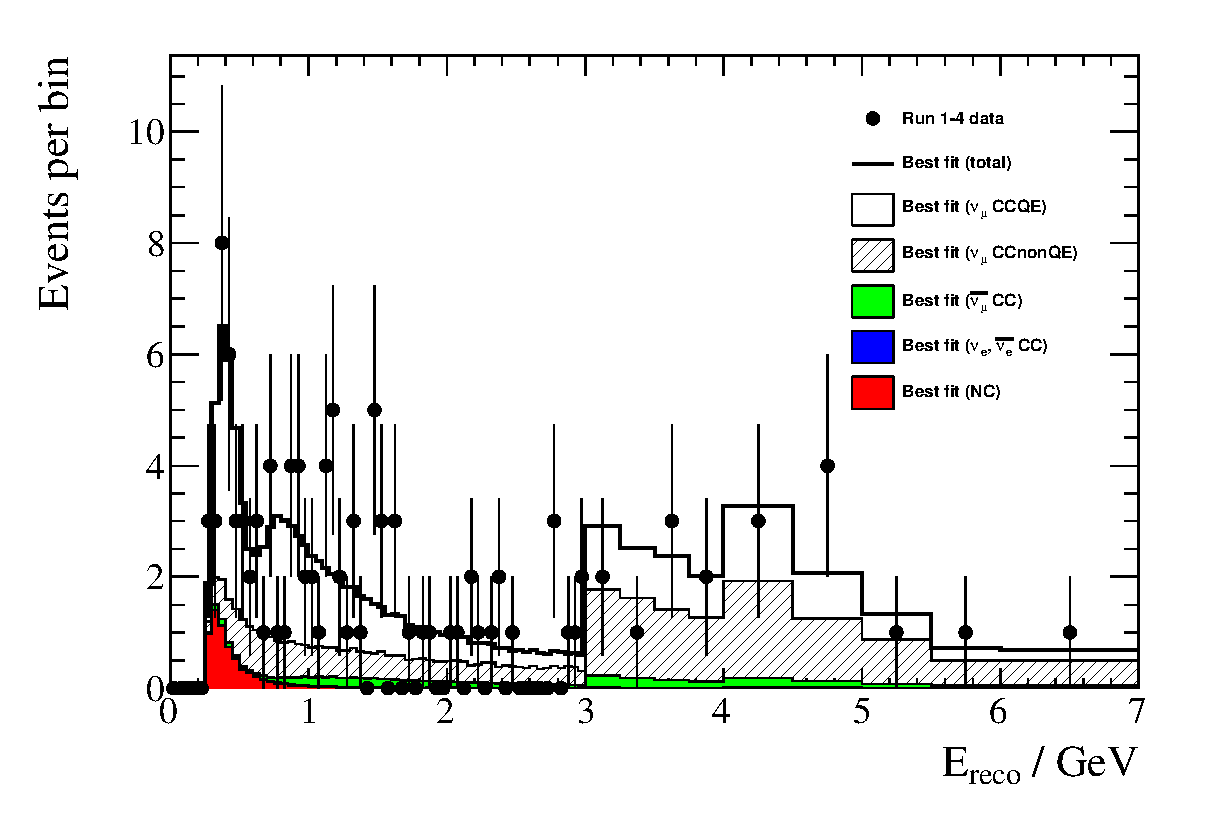
\includegraphics[width=24pc]{./images/data_results/run1234a_normal/run1-4_nuis3fixdcp_sintheta_normal_spectrum_components}
  \caption {
    Best-fit reconstructed energy spectrum in the 73-bin scheme used in the fit (see Sec.\ 2.2.5 in 
    Ref.\ \cite{OurRun123DisappAnalysis3Flavour}) and its components
    obtained from the fit to the Run 1+2+3+4a dataset.  
    The 32 components, each of which is calculated separately, are grouped into just 5 categories:
    $\nu_{\mu}$ CCQE, $\nu_{\mu}$ CCnQE, $\bar{\nu_{\mu}}$ CC, $\nu_{e}$/$\bar{\nu_{e}}$ CC and NC.  
    The normal mass hierarchy is assumed.
  }
  \label{fig:results_data1234a_spectrum_components:normal}
\end{figure*}

\begin{figure*}[htb]
  \center
  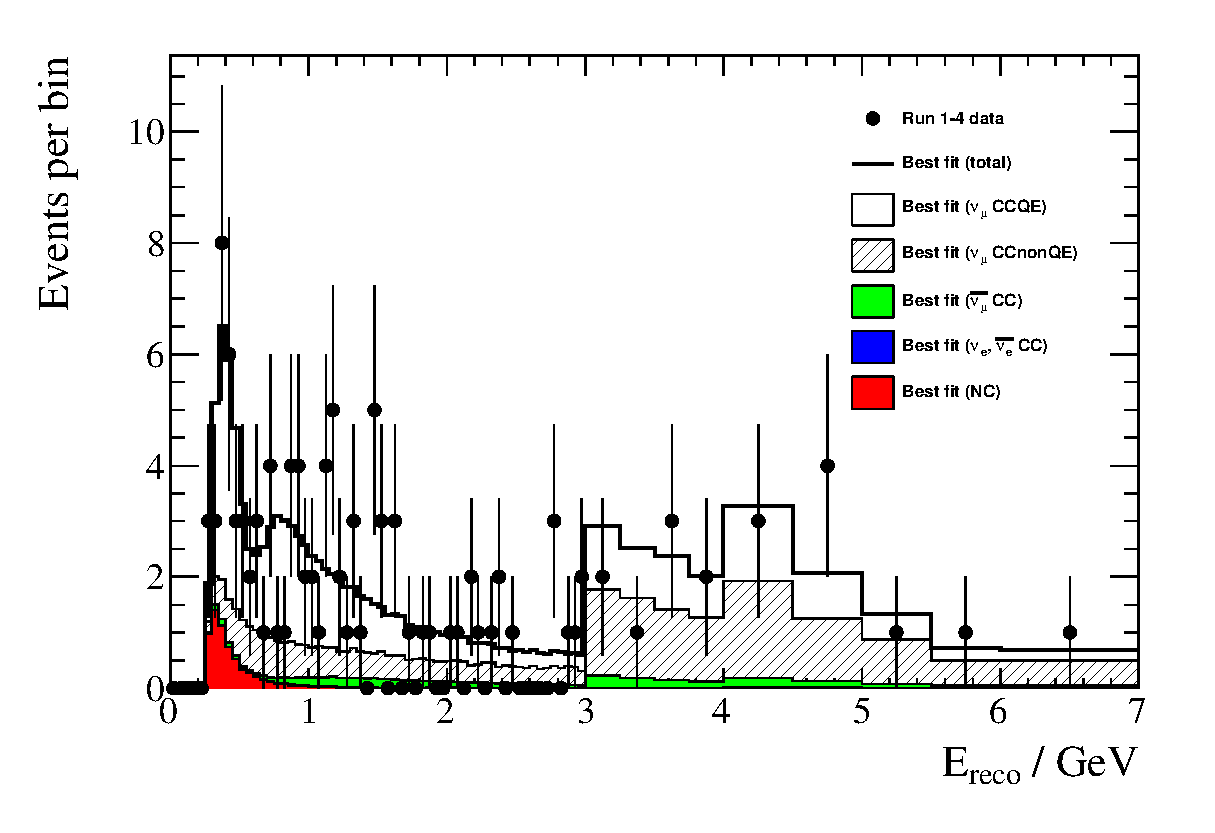
\includegraphics[width=24pc]{./images/data_results/run1234a_inverted/run1-4_nuis3fixdcp_sintheta_inverted_spectrum_components}
  \caption {
    Best-fit reconstructed energy spectrum in the 73-bin scheme used in the fit (see Sec.\ 2.2.5 in 
    Ref.\ \cite{OurRun123DisappAnalysis3Flavour}) and its components
    obtained from the fit to the Run 1+2+3+4a dataset.  
    The 32 components, each of which is calculated separately, are grouped into just 5 categories:
    $\nu_{\mu}$ CCQE, $\nu_{\mu}$ CCnQE, $\bar{\nu_{\mu}}$ CC, $\nu_{e}$/$\bar{\nu_{e}}$ CC and NC.  
    The inverted mass hierarchy is assumed.
  }
  \label{fig:results_data1234a_spectrum_components:inverted}
\end{figure*}


%...........................................................
%
% Best-fit spectra comparisons between normal & inverted hierarchy (73 bin and coarse binning)
%
\begin{figure*}[htb]
\center
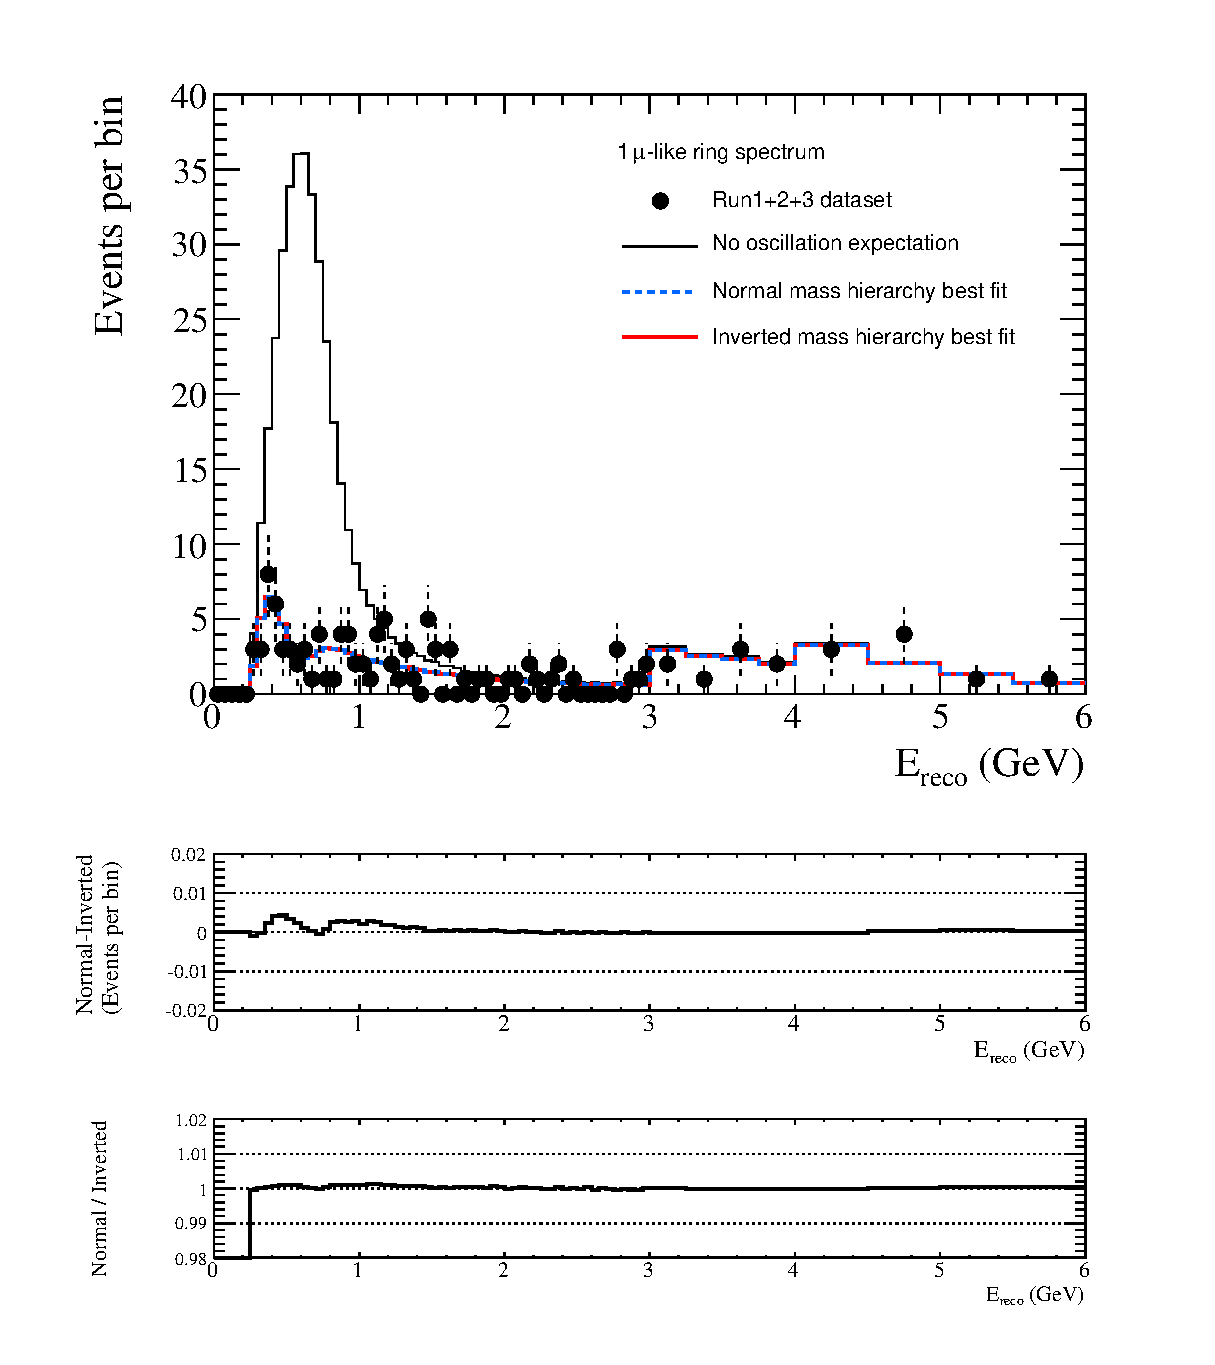
\includegraphics[width=40pc]{./images/data_results/compare/spectrum_comparison_normal_inverted}
\caption {
  Comparison between best-fit reconstructed energy spectra
  obtained from the normal and inverted mass hierarchy fits to the Run 1+2+3+4a datasets.
  The spectra are shown using the 73 bins used in the fit (see Sec.\ 2.2.5 in 
  Ref.\ \cite{OurRun123DisappAnalysis3Flavour}).
  Also shown are the absolute difference between the normal and inverted mass hierarchy
  best-fit spectra and 
  the ratio between them.
}
\label{fig:results_data1234a_spectrum_comparison}
\end{figure*}

\begin{figure*}[htb]
\center
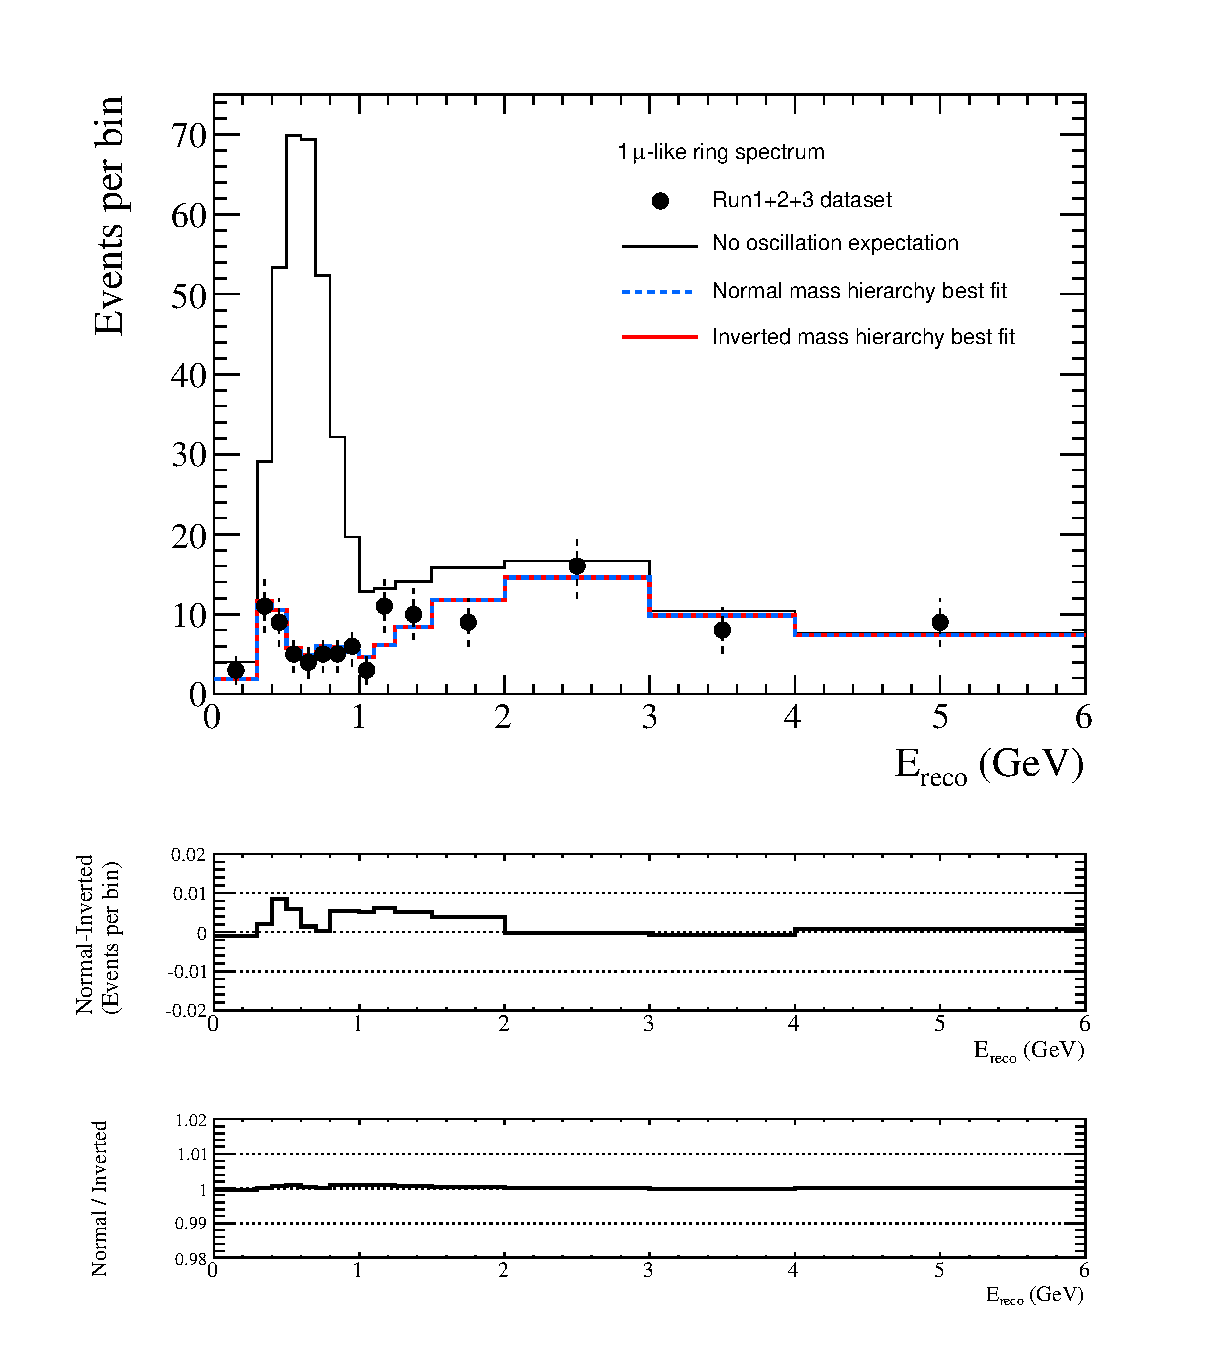
\includegraphics[width=40pc]{./images/data_results/compare/spectrum_comparison_normal_inverted_coarse}
\caption {
  Comparison between best-fit reconstructed energy spectra
  obtained from the normal and inverted mass hierarchy fits to the Run 1+2+3+4a datasets.
  The spectra are shown using the coarse binning scheme discussed in the text (see Sec.\ \ref{sec:results_bestfit_spectra}).
  Also shown are the absolute difference between the normal and inverted mass hierarchy
  best-fit spectra and 
  the ratio between them.
}
\label{fig:results_data1234a_spectrum_comparison_coarse}
\end{figure*}


%--------------------------------------------------------------------------------------
% Contours
%--------------------------------------------------------------------------------------

\clearpage

\subsection {Confidence regions}
\label{sec:results_contours}

The first step in constructing confidence contours in the 2-dimensional ($\sin^{2}\theta_{23}$, $|\Delta m^{2}_{32}|$)
oscillation parameter space is to construct the $\Delta\chi^2$ surface in that space.
The oscillation parameter space is divided into a rectangular grid of width $\sin^{2}\theta_{23}$ = 0.005, $|\Delta m^{2}_{32}|$ = 
0.05$\times$10$^{-3}$ eV$^{2}$/c$^{4}$, with a grid point at the centre of each rectangle. Two separate fits are made of 
the data at each grid point: in one fit, the values of $\sin^{2}\theta_{23}$ and $|\Delta m^{2}_{32}|$ are fixed to the true 
values of the grid point and the 44 systematic parameters are allowed to float, while in the other fit $\sin^{2}\theta_{23}$, 
$|\Delta m^{2}_{32}|$ and the 44 systematic parameters are allowed to float. $\delta_{CP}$ is fixed at 0 in both fits.
$\Delta\chi^2$ is then calculated as the 
difference between the minimum values of $\chi^{2}$ from the two fits ($\chi^{2}$ is defined in Eq.\ 5 in Sec.\ 4.1.5 
in Ref.\ \cite{OurRun123DisappAnalysis3Flavour}).

The 2-dimensional $\Delta\chi^2$ surface for the fit to the Run 1+2+3+4a dataset is shown in
Figs.\ \ref{fig:results_data1234a_chisq:normal} and \ref{fig:results_data1234a_chisq:inverted}
as a function of $\sin^{2}\theta_{23}$ and $|\Delta m^{2}_{32}|$,
for the normal and inverted mass hierarchies respectively.
% For comparison, the corresponding $\Delta\chi^2$ surfaces for the fits to the Run 1+2+3 and Run 4a
% datasets are shown in Figs.\ \ref{fig:results_data123_chisq} and \ref{fig:results_data4a_chisq} respectively.
The same $\Delta\chi^2$ range is used in both %all
colour plots to allow comparison.
Profile $\Delta\chi^2$ distributions are also shown as a function of $\sin^{2}\theta_{23}$ 
and $|\Delta m^{2}_{32}|$ for the %fits to the Run 1+2+3+4a, Run 1+2+3 and Run 4a datasets in
fit to the Run 1+2+3+4a dataset in 
%Figs.\ \ref{fig:results_marg_dchisq_dmsq_all3} and \ref{fig:results_marg_dchisq_sinsq_all3} respectively.
Figs.\ \ref{fig:results_marg_dchisq_dmsq_normalinverted} and \ref{fig:results_marg_dchisq_sinsq_normalinverted} respectively.
Using these plots and the constant-$\Delta\chi^2$ method described in Sec.\ 5.4 of Ref.\ \cite{OurRun123DisappAnalysis3Flavour},
1-dimensional limits on the parameters can be obtained\footnote{
For 1 fit parameter, the critical values of $\Delta{\chi^{2}}$ used are 
1.00 (68\% CL), 2.71 (90\% CL), 3.84 (95\% CL), 6.63 (99\% CL).
For 2 parameters fitted simultaneously, the critical values of $\Delta{\chi^{2}}$ used are 
2.30 (68\% CL), 4.61 (90\% CL), 5.99 (95\% CL), 9.21 (99\% CL).
}.
These limits are presented in Tab.\ \ref{tab:data_fits:1dlimits}.

2-dimensional confidence regions were constructed
for the %fits to the Run 1+2+3+4a, Run 1+2+3 and Run 4a datasets
fit to the Run 1+2+3+4a dataset 
using the constant-$\Delta\chi^2$ method described in 
Sec.\ 4.5 of Ref.\ \cite{OurRun123DisappAnalysis3Flavour}.
The 68\% and 90\% CL regions for the fit to the Run 1+2+3+4a dataset are shown 
in Figs.\ \ref{fig:results_data1234a_contour:normal} and \ref{fig:results_data1234a_contour:inverted}
for the normal and inverted mass hierarchies respectively.
% The corresponding constant-$\Delta\chi^2$ contours for the Run 1+2+3 and Run 4a datasets are shown 
% in Figs.\ \ref{fig:results_data123_contour} and \ref{fig:results_data4a_contour} respectively. 
All confidence regions presented include the effect of systematic uncertainties.

To construct 2-dimensional confidence regions using the method of Feldman and Cousins \cite{FeldmanCousins},
described in Sec.\ 4.5 of Ref.\ \cite{OurRun123DisappAnalysis3Flavour}, 
one needs to construct $\Delta\chi^{2}_{critical}$ surfaces,
in the ($\sin^{2}\theta_{23}$, $|\Delta m^{2}_{32}|$) oscillation parameter space,
for the $6.3933 \times 10^{20}$-POT 3-flavour $\nu_{\mu}$-disappearance analysis.
At each grid point, an ensemble of toy MC experiments is created with $\sin^{2}\theta_{23}$ and $|\Delta m^{2}_{32}|$
set to the true values of that grid point and all 44 systematic parameters randomized ($\delta_{CP}$ is also randomized uniformly between $-\pi$ and $+\pi$).
Each toy experiment 
is fitted twice: again in the first fit the values of $\sin^{2}\theta_{23}$ and $|\Delta m^{2}_{32}|$ are fixed to the true
values of the grid point and the 44 systematic parameters are allowed to float, while in the 
second fit $\sin^{2}\theta_{23}$, $|\Delta m^{2}_{32}|$ and the 44 systematic parameters are allowed to 
float. This means that $\chi^{2}$ is {\em independently} minimised for {\em each} toy MC experiment with respect 
to the systematic parameters. For each toy MC experiment, $\Delta\chi^2$ is given by the difference between the 
minimum values of $\chi^{2}$ from the two fits (the first fit gives the ``true'' $\chi^{2}$ and the 
second fit gives the ``best-fit'' $\chi^{2}$). The value of $\Delta\chi^{2}_{critical}$ for a grid 
point is the value of $\Delta\chi^2$ such that $\alpha$ of the toy experiments at that grid point have 
$\Delta\chi^2$ $<$ $\Delta\chi^{2}_{critical}$, where $\alpha$ is the desired confidence level.  

In Fig.\ \ref{fig:fc_dchisqcrit_2d:normal}, we show a Monte Carlo estimation using the Feldman-Cousins method
of the 2-dimensional $\Delta\chi^{2}_{critical}$ values
used for calculation of the 68\% and 90\% CL confidence regions,
assuming the normal mass hierarchy.
The surfaces were generated using an ensemble of toy MC experiments which included both
randomized systematic variations and statistical fluctuations.
Slices of the 2-dimensional distributions shown in Fig.\ \ref{fig:fc_dchisqcrit_2d:normal},
are shown in Figs.\ \ref{fig:fc_dchisqcrit_slice_mixing:normal} and \ref{fig:fc_dchisqcrit_slice_dmsq:normal}.
From these $\Delta\chi^{2}_{critical}$ distributions, we anticipate that the confidence regions produced
using the Feldman-Cousins method will be narrower along $|\Delta{m^{2}_{32}}|$ at maximal mixing than
those made with the constant-$\Delta\chi^{2}$ method. The Feldman-Cousins contours will also be wider
in $\sin^{2}{\theta_{23}}$ for values of $|\Delta{m^{2}_{32}}|$ near the best fit.
This is the same pattern that was seen by our previous analyses 
\cite{OurRun12DisappAnalysis,OurRun123DisappAnalysis3Flavour} that fit for
$\sin^2(2\theta_{23})$.

Using the $\Delta\chi^2$ and $\Delta\chi^{2}_{critical}$ surfaces presented here,
the 2-dimensional Feldman-Cousins 68\% and 90\% CL regions were constructed 
and they are shown in Fig.\ \ref{fig:results_data1234a_fc_contour:normal}.
Due to the large amount of CPU time needed to generate the contours with the complete 2013 VaLOR analysis,
the Feldman-Cousins confidence regions are currently shown
only for the normal mass hierarchy;
the inverted mass hierarchy confidence regions will be prepared at a later date.
% only for the fit to the combined Run 1+2+3+4a dataset.
All confidence regions presented include the effect of systematic uncertainties.

Confidence intervals were also constructed using the method of Feldman and Cousins in each of $\sin^2 \theta_{23}$ and $
\Delta m_{32}^{2}$ separately. To make the 1-dimensional confidence interval in $\sin^2 \theta_{23}$, an ensemble of 
toy MC experiments is generated, and each experiment is fitted twice. In the first fit, $\Delta m_{32}^{2}$ and 
all 44 systematic parameters are allowed to float, while $\sin^2 \theta_{23}$ is fixed to the true input value 
for that experiment. In the second fit, $\sin^2 \theta_{23}$, $\Delta m_{32}^{2}$ and all 44 systematic parameters 
are allowed to float. Again this means that $\chi^{2}$ is independently minimised with respect to the systematic 
parameters for each toy MC experiment. The value of $\Delta\chi^{2}$ is given by the difference between the 
minimum values of $\chi^{2}$ from the two fits for each experiment. 

One issue in constructing these 1-dimensional confidence intervals concerns the choice of the true input value(s) of the 
``other'' oscillation parameter in the toy MC experiments. For example, true input values of $\Delta m_{32}^{2}$ must be 
chosen when making the toy experiments for the confidence interval in $\sin^2 \theta_{23}$. One option in this case would 
be to use the T2K Run 1+2+3+4a best-fit value of $\Delta m_{32}^{2}$ as the true input value for all the toy MC experiments, 
but this fails to account for the uncertainty in $\Delta m_{32}^{2}$. Alternatively, a uniform distribution of true input 
values of $\Delta m_{32}^{2}$ could be used in some range, say from 2-3$\times$10$^{-3}$eV$^{2}$/c$^{4}$, but this ignores 
the fact that some values of $\Delta m_{32}^{2}$ are preferred by the T2K Run 1+2+3+4a data to others. 

In this analysis, the true input values of $\Delta m_{32}^{2}$ are chosen using the likelihood from the 2-dimensional fit of 
the T2K Run 1+2+3+4a data in $\sin^2 \theta_{23}$ and $\Delta m_{32}^{2}$ and the 44 nuisance parameters. Since the value of 
$\chi^{2}$ for this fit, as defined in equation 3 in Sec.\ 4.1.5 in Ref.\ \cite{OurRun123DisappAnalysis3Flavour}, is -2 ln(likelihood), 
the likelihood is e$^{-\frac{\chi^{2}}{2}}$; this likelihood is equal to a constant times e$^{-\frac{\Delta \chi^{2}}{2}}$ as the 
best-fit value of $\chi^{2}$ is constant. At each true value of $\sin^2 \theta_{23}$, toy MC experiments are made with different 
true input values of $\Delta m_{32}^{2}$, and the numbers of experiments with each input value of $\Delta m_{32}^{2}$ are 
chosen to be proportional to e$^{-\frac{\Delta \chi^{2}}{2}}$, where $\Delta \chi^{2}$ is the value of the 2-dimensional 
$\Delta \chi^{2}$ surface in Fig.\ \ref{fig:results_data1234a_chisq:normal} or Fig.\ \ref{fig:results_data1234a_chisq:inverted} 
at those values of $\sin^2 \theta_{23}$ and $\Delta m_{32}^{2}$. 

The critical value of $\Delta \chi^{2}$ at each true value of $\sin^2 \theta_{23}$ is found by combining all the toy MC 
experiments with that input value of $\sin^2 \theta_{23}$ and different true input values of $\Delta m_{32}^{2}$. It is the value 
of $\Delta \chi^{2}$ such that $\alpha$ of the toy experiments have $\Delta \chi^{2}$ $<$ $\Delta \chi^{2}_{critical}$, 
where $\alpha$ is the desired confidence level. 

The 1-dimensional confidence intervals in $\Delta m_{32}^{2}$ are constructed in a similar way. At each true value of 
$\Delta m_{32}^{2}$, the numbers of toy MC experiments with each input value of $\sin^2 \theta_{23}$ are proportional to 
e$^{-\frac{\Delta \chi^{2}}{2}}$, while all of them have that value of $\Delta m_{32}^{2}$ as input. Again each experiment 
is fitted twice: in the first fit, $\sin^2 \theta_{23}$ and all 44 systematic parameters are allowed to float with  
$\Delta m_{32}^{2}$ fixed at its true input value, whereas, in the second fit, $\Delta m_{32}^{2}$, $\sin^2 \theta_{23}$ 
and all 44 systematic parameters are allowed to float. For each experiment, the value of $\Delta \chi^{2}$ is the difference 
between the values of $\chi^{2}$ from the two fits. The critical value of $\Delta \chi^{2}$ at each true value of 
$\Delta m_{32}^{2}$ is found by combining all the experiments with that input value of $\Delta m_{32}^{2}$ and different 
input values of $\sin^2 \theta_{23}$.

In the next section, comparisons are presented of the confidence regions obtained 
using different construction methods.
We also compare our contours from the fit to the combined Run 1+2+3+4a dataset
with recent measurements from MINOS and SuperK.
% The contours from different running periods are compared, and we also compare our contours
% from the fit to the combined Run 1+2+3+4a dataset with recent measurements from MINOS and 
% SuperK and T2K 6.3933$\times$10$^{20}$-POT sensitivity contours. 


%...........................................................
%
% \Delta\chisquare surfaces 
%
\begin{figure*}[htb]
\center
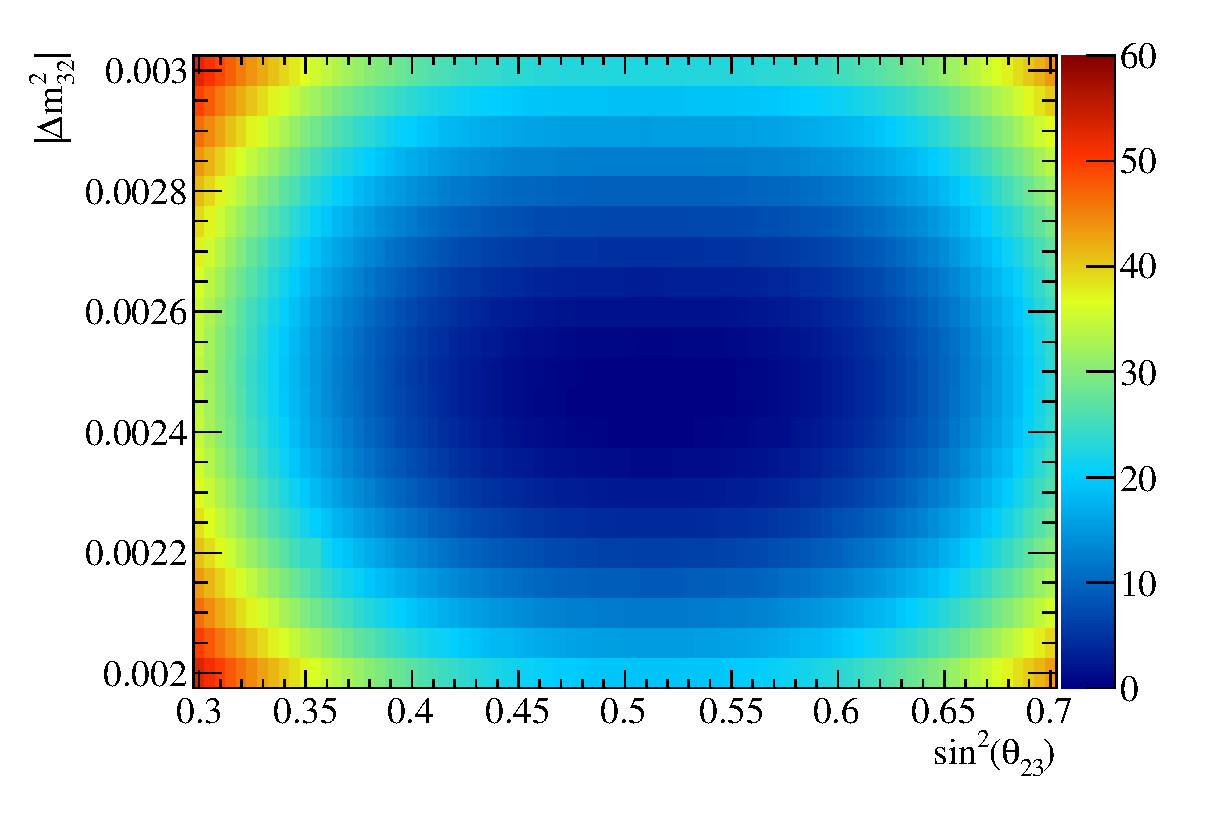
\includegraphics[width=36pc]{./images/data_results/run1234a_normal/run1-4_nuis3fixdcp_sintheta_normal_dchisq_maxz60}
\caption {
  $\Delta\chi^2$ surface for the fit to the Run 1+2+3+4a dataset.
  The normal mass hierarchy is assumed.
}
\label{fig:results_data1234a_chisq:normal}
\end{figure*}

\begin{figure*}[htb]
\center
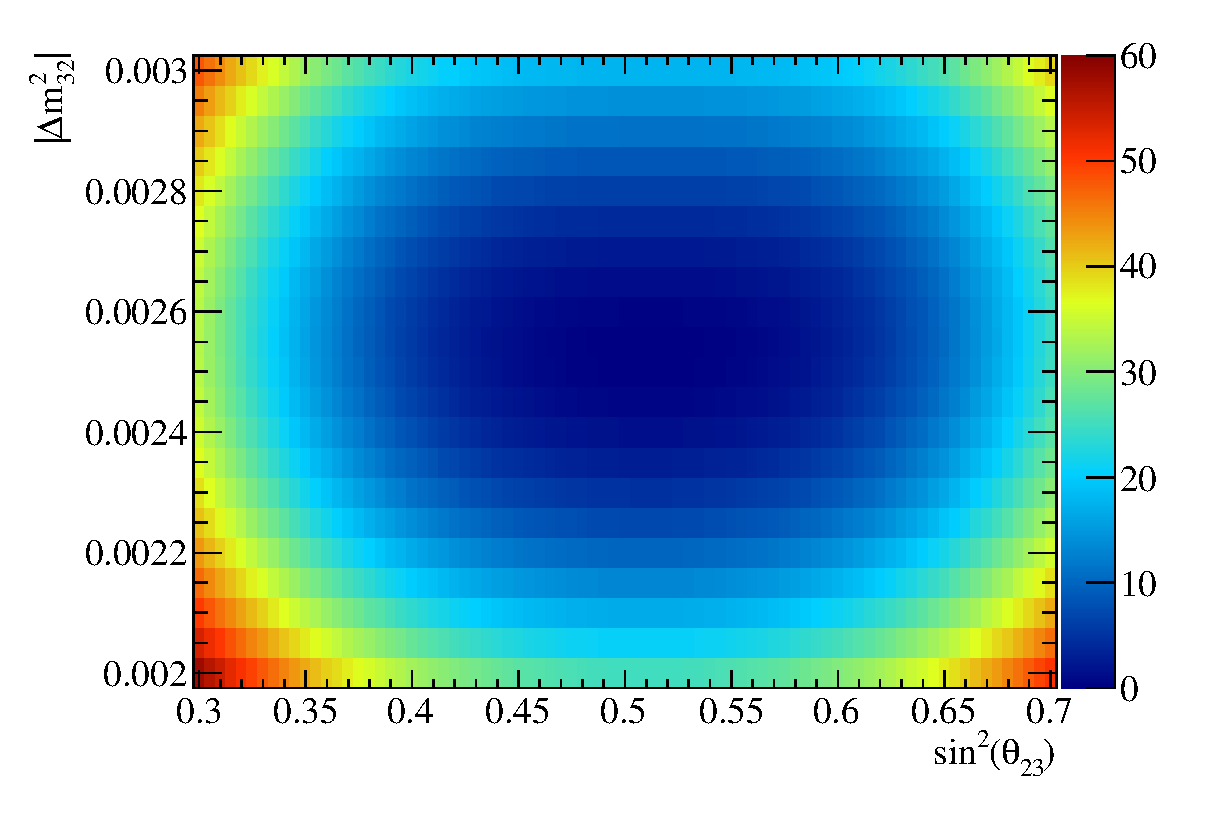
\includegraphics[width=36pc]{./images/data_results/run1234a_inverted/run1-4_nuis3fixdcp_sintheta_inverted_dchisq_maxz60}
\caption {
  $\Delta\chi^2$ surface for the fit to the Run 1+2+3+4a dataset.
  The inverted mass hierarchy is assumed.
}
\label{fig:results_data1234a_chisq:inverted}
\end{figure*}


% \begin{figure*}[htb]
% \begin{minipage}[t]{0.48\linewidth}
% \center
% 
\includegraphics[width=21pc]{./images/placeholder.eps}
% \caption {
%   $\Delta\chi^2$ surface for the fit to the Run 1+2+3 dataset.
% }
% \label{fig:results_data123_chisq}
% \end{minipage}
% \hspace{0.06\linewidth}
% \begin{minipage}[t]{0.48\linewidth}
% \center
% 
\includegraphics[width=21pc]{./images/placeholder.eps}
% \caption {
%   $\Delta\chi^2$ surface for the fit to the Run 4a dataset.
% }
% \label{fig:results_data4a_chisq}
% \end{minipage}
% \end{figure*}

\clearpage

%...........................................................
%
% Marginalised \Delta\chisquare plots & Table summarizing 1D limits
%

% \begin{figure*}[htb]
% \center
% 
\includegraphics[width=35pc]{./images/placeholder.eps}
% \caption {
%   Profile $\Delta\chi^2$, as a function of $|\Delta m^{2}_{32}|$, 
%   for the three fits to the Run 1+2+3+4a, Run 1+2+3 and Run 4a datasets.
% }
% \label{fig:results_marg_dchisq_dmsq_all3}
% \end{figure*}

% \begin{figure*}[htb]
% \center
% 
\includegraphics[width=35pc]{./images/placeholder.eps}
% \caption {
%   Profile $\Delta\chi^2$, as a function of $\sin^{2}\theta_{23}$, 
%   for the three fits to the Run 1+2+3+4a, Run 1+2+3 and Run 4a datasets.
% }
% \label{fig:results_marg_dchisq_sinsq_all3}
% \end{figure*}


\begin{figure*}[htb]
  \begin{minipage}[t]{0.96\linewidth}
    \center
    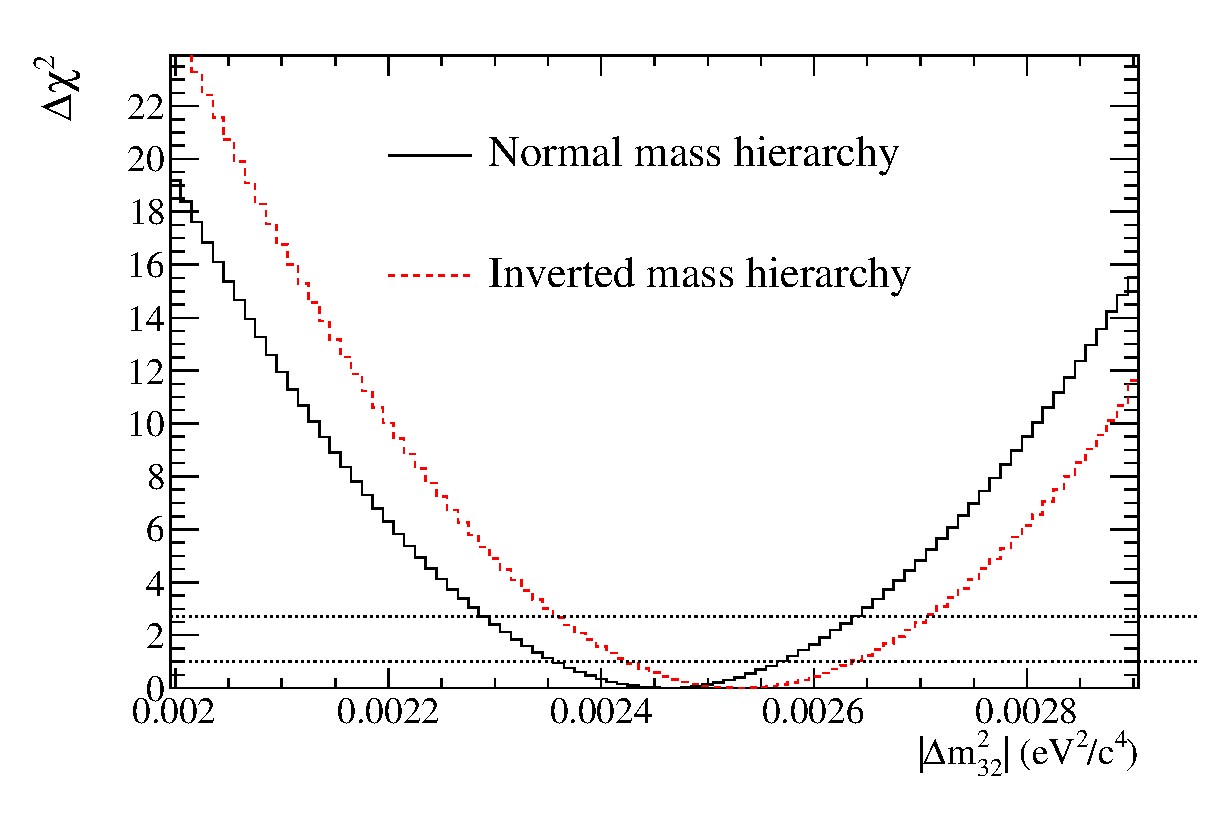
\includegraphics[width=30pc]{./images/data_results/compare/dchisq_profiles_dm32sq}
    \caption {
      Profile $\Delta\chi^2$, as a function of $|\Delta m^{2}_{32}|$, 
      for the fits to the Run 1+2+3+4a dataset
      assuming normal and inverted mass hierarchy.
      The 68\% and 90\% constant-$\Delta\chi^{2}$ values
      are shown as horizontal dotted lines.
    }
    \label{fig:results_marg_dchisq_dmsq_normalinverted}
  \end{minipage}
  \vfill
  \begin{minipage}[t]{0.96\linewidth}
    \center
    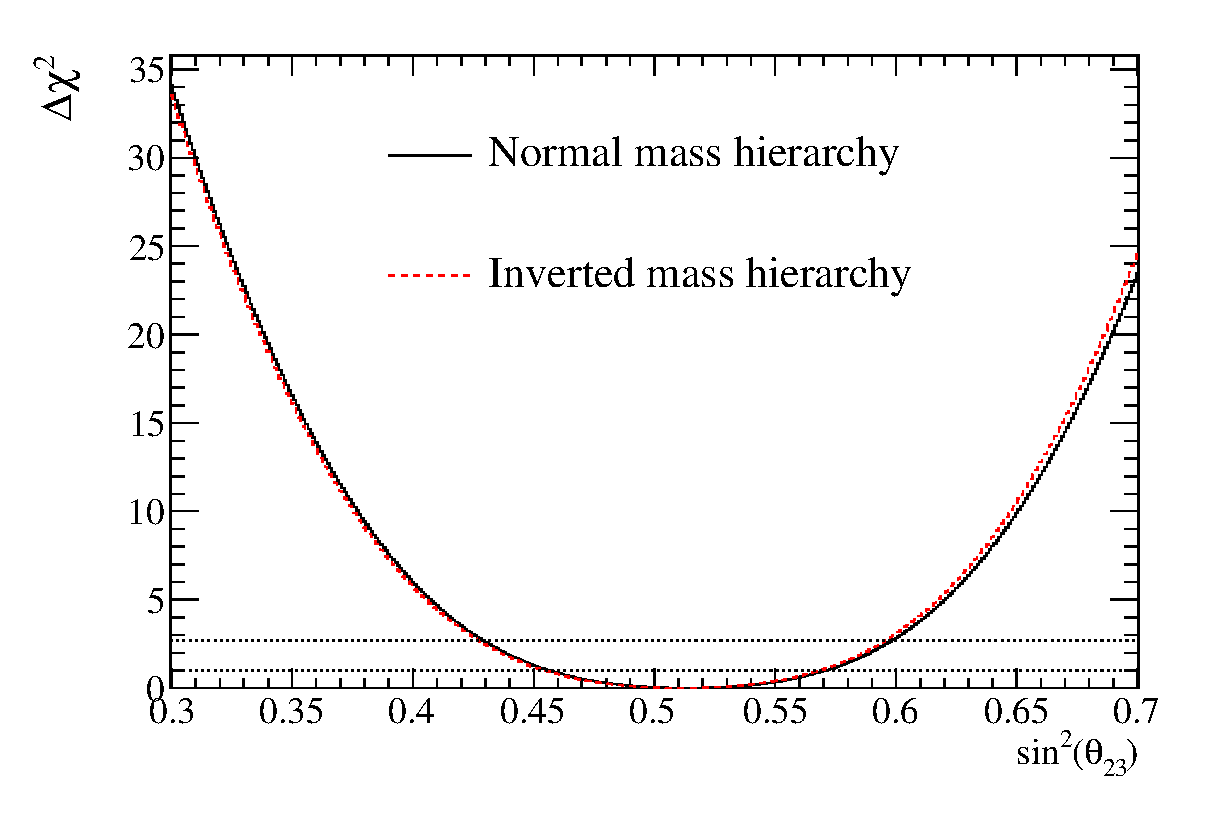
\includegraphics[width=30pc]{./images/data_results/compare/dchisq_profiles_mix23}
    \caption {
      Profile $\Delta\chi^2$, as a function of $\sin^{2}\theta_{23}$, 
      for the fits to the Run 1+2+3+4a dataset
      assuming normal and inverted mass hierarchy.
      The 68\% and 90\% constant-$\Delta\chi^{2}$ values
      are shown as horizontal dotted lines.
    }
    \label{fig:results_marg_dchisq_sinsq_normalinverted}
  \end{minipage}
  \vfill
  \begin{minipage}[t]{0.96\linewidth}
    \centering
    \begin{tabular}{| l | l | c | D{.}{.}{-1} D{.}{.}{-1} | D{.}{.}{-1}  D{.}{.}{-1} |}
      \hline
      Analysis & Run period & Limit & \multicolumn{2}{c|}{$\sin^{2}\theta_{23}$}
      &  \multicolumn{2}{c|}{$\Delta m_{32}^2$ / $\cdot 10^{-3}$ eV$^2$/c$^4$} \\
      \hline
      2013 3-flavour Normal   & Run 1+2+3+4a & 68\% & >0.456 & <0.572 & >2.35 & <2.57 \\
      2013 3-flavour Normal   & Run 1+2+3+4a & 90\% & >0.428 & <0.599 & >2.29 & <2.64 \\
      2013 3-flavour Inverted & Run 1+2+3+4a & 68\% & >0.454 & <0.569 & >2.42 & <2.64 \\
      2013 3-flavour Inverted & Run 1+2+3+4a & 90\% & >0.426 & <0.596 & >2.35 & <2.71 \\
      \hline
    \end{tabular}
    \captionof{table}{
      %\caption{
      Summary of one-dimensional limits on $\sin^{2}\theta_{23}$ and $\Delta m_{32}^2$,
      for the oscillation fits to the Run 1+2+3+4a dataset.
      The limits are calculated using the constant-$\Delta\chi^2$ method.
    }
    \label{tab:data_fits:1dlimits}
  \end{minipage}
\end{figure*}

%...........................................................
%
% Const-dchi^2 contours 
%
\begin{figure*}[htb]
\center
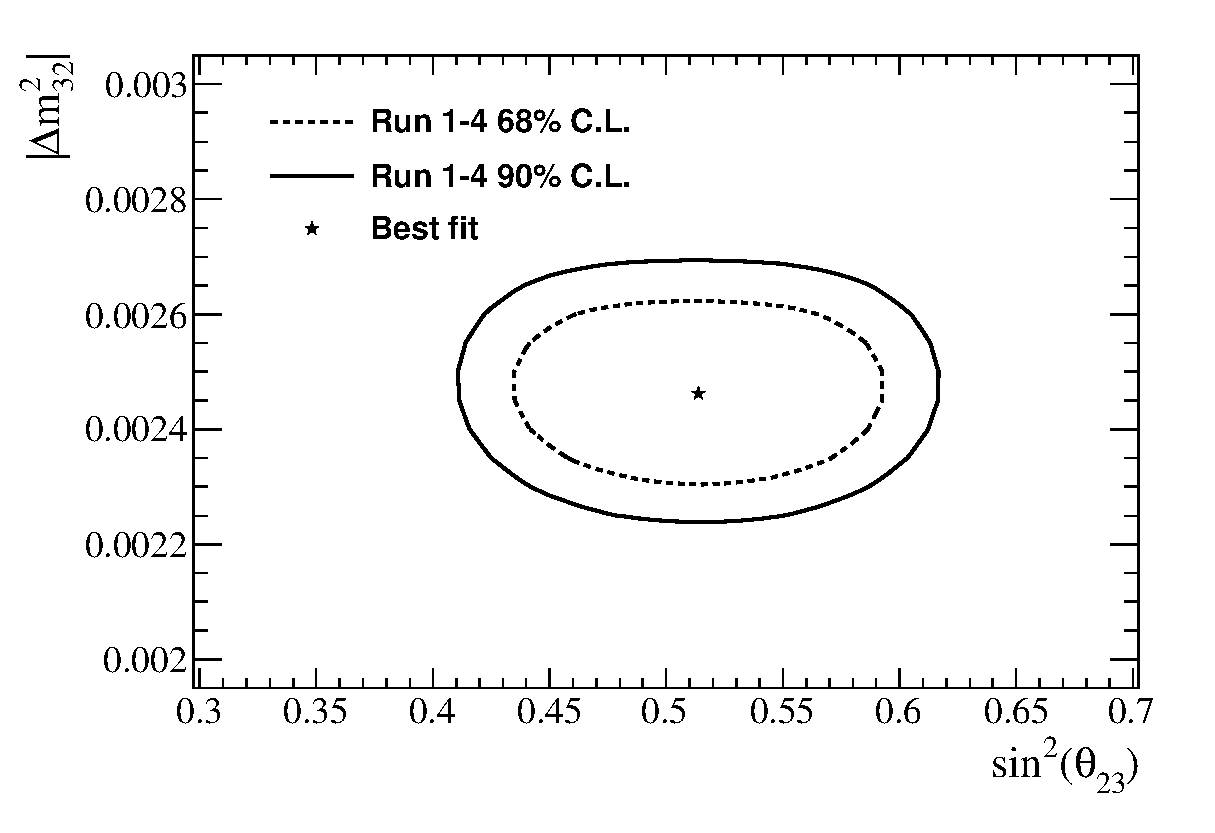
\includegraphics[width=35pc]{./images/data_results/run1234a_normal/run1-4_nuis3fixdcp_sintheta_normal_contour}
\caption {
  68\% CL and 90\% CL allowed region (including systematics), 
  constructed with the constant-$\Delta\chi^{2}$ method,
  for the fit to the Run 1+2+3+4a dataset.
  The best-fit point is also shown.
  The normal mass hierarchy is assumed.
}
\label{fig:results_data1234a_contour:normal}
\end{figure*}

\begin{figure*}[htb]
\center
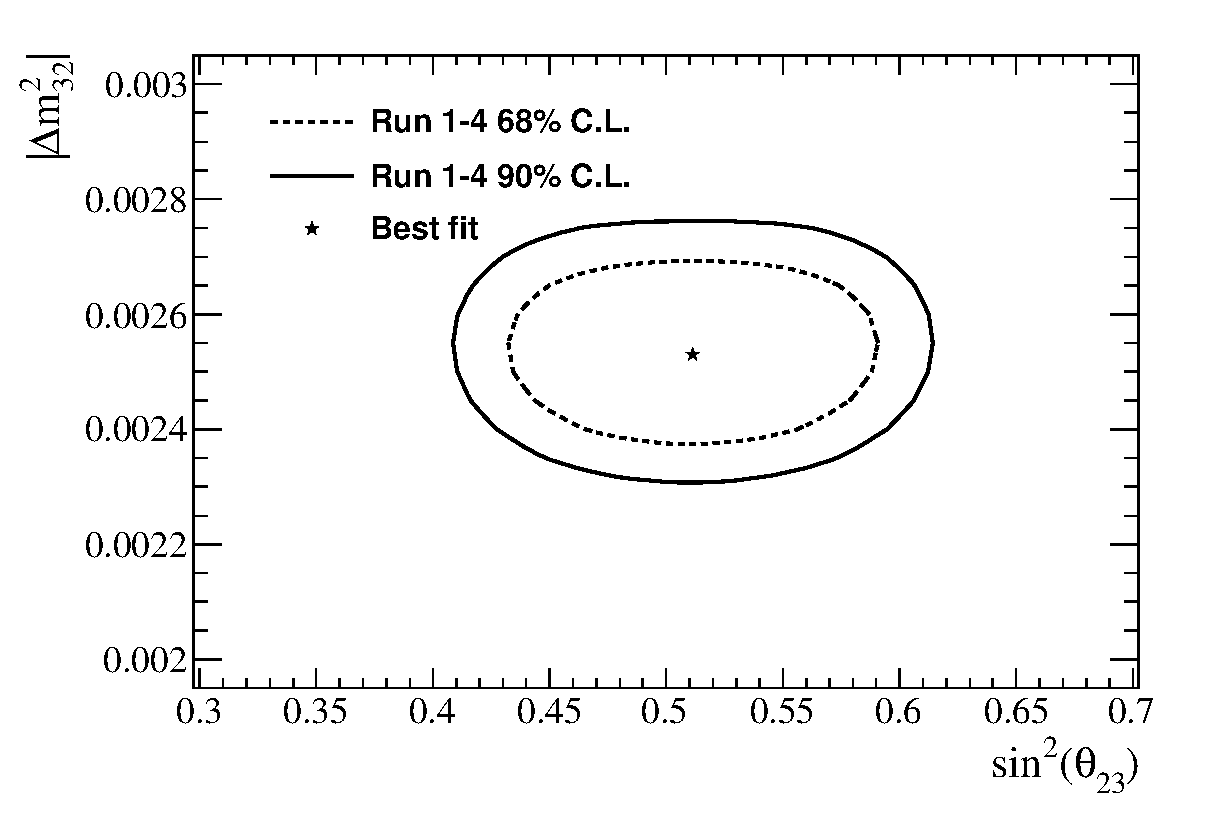
\includegraphics[width=35pc]{./images/data_results/run1234a_inverted/run1-4_nuis3fixdcp_sintheta_inverted_contour}
\caption {
  68\% CL and 90\% CL allowed region (including systematics), 
  constructed with the constant-$\Delta\chi^{2}$ method,
  for the fit to the Run 1+2+3+4a dataset.
  The best-fit point is also shown.
  The inverted mass hierarchy is assumed.
}
\label{fig:results_data1234a_contour:inverted}
\end{figure*}

% \begin{figure*}[htb]
% \begin{minipage}[t]{0.48\linewidth}
% \center
% 
\includegraphics[width=20pc]{./images/placeholder.eps}
% \caption {
%   As in Fig.\ \ref{fig:results_data1234a_contour}, but for the Run 1+2+3 dataset only.
% }
% \label{fig:results_data123_contour}
% \end{minipage}
% \hspace{0.06\linewidth}
% \begin{minipage}[t]{0.48\linewidth}
% \center
% 
\includegraphics[width=20pc]{./images/placeholder.eps}
% \caption {
%   As in Fig.\ \ref{fig:results_data1234a_contour}, but for the Run 4a dataset only.
% }
% \label{fig:results_data4a_contour}
% \end{minipage}
% \end{figure*}

%...........................................................
%
% FC dchisq_critical surfaces
%

\begin{figure*}[htb]
\center
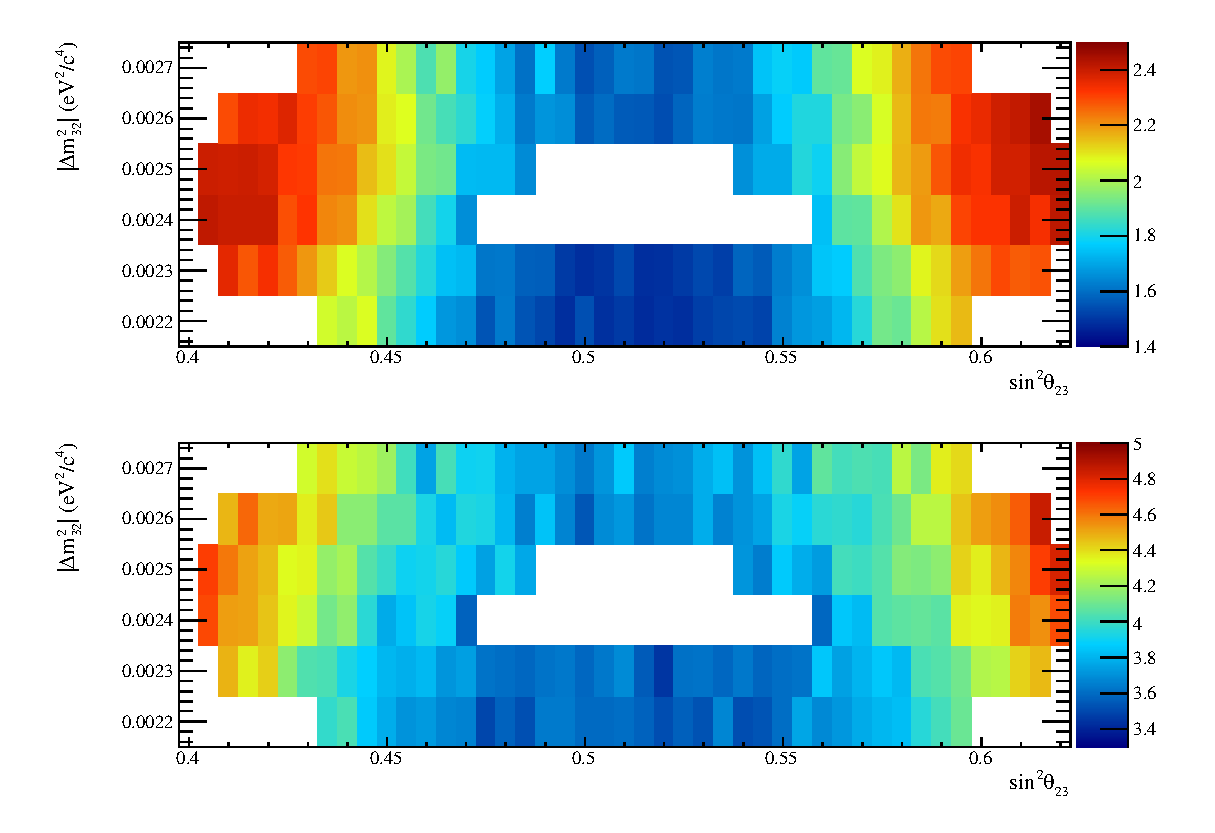
\includegraphics[width=42pc]{./images/fc_surface/FC_surfaces}
\caption {
  Monte Carlo estimation,
  according to the method of Feldman and Cousins \cite{FeldmanCousins},
  of $\Delta\chi^{2}_{critical}$ values $\Delta\chi^{2}_{68}$ (left) and $\Delta\chi^{2}_{90}$ (right)
  as a function of $\sin^{2}{\theta_{23}}$ and $|\Delta{m^{2}_{32}}|$,
  for calculation of the 68\% and 90\% CL confidence regions
  for the 6.3933 $\times$10$^{20}$-POT 3-flavour $\nu_{\mu}$-disappearance analysis.
  The surfaces were generated from an ensemble of toy MC experiments including both
  randomized systematic variations and statistical fluctuations.
  As expected from \cite{FeldmanCousins}, the values of $\Delta\chi^{2}_{critical}$
  decrease as the limit of the model at $\sin^{2}{\theta_{23}} \approx 0.513$ is approached.
  The normal mass hierarchy is assumed.
  It should be noted that $\Delta\chi^2_{critical}$ is not calculated for every combination of
  $\sin^{2}{\theta_{23}}$ and $|\Delta{m^{2}_{32}}|$,
  due to us being efficient with computing time.
}
\label{fig:fc_dchisqcrit_2d:normal}
\end{figure*}

%.......

\begin{figure*}[htb]
\center
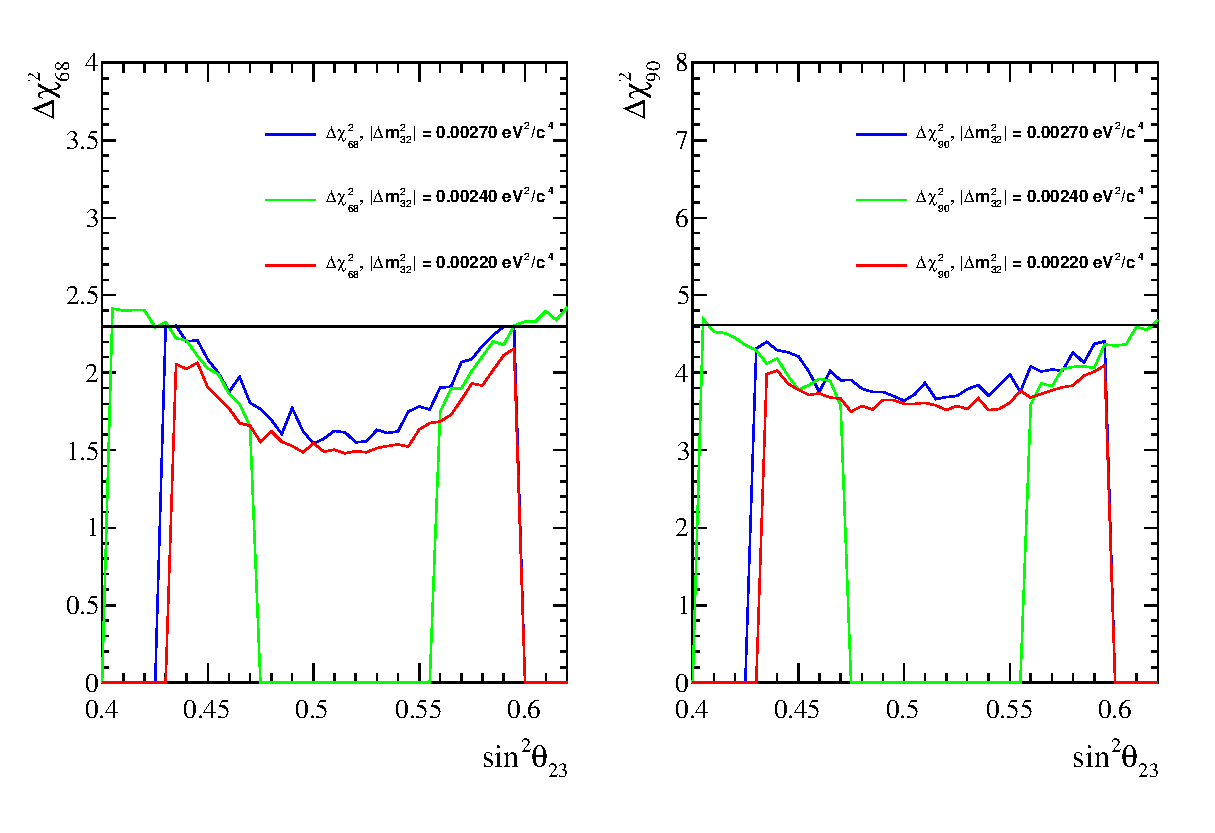
\includegraphics[width=30pc]{./images/fc_surface/FC_slice_mixing}
\caption {
  Monte Carlo estimation,
  according to the method of Feldman and Cousins,
  of $\Delta\chi^{2}_{critical}$ values $\Delta\chi^{2}_{68}$ (left) and $\Delta\chi^{2}_{90}$ (right),
  as a function of $\sin^{2}{\theta_{23}}$ for 3 different values of $|\Delta{m^{2}_{32}}|$
  (2.2$\times$10$^{-3}$ eV$^{2}/c^{4}$,
   2.4$\times$10$^{-3}$ eV$^{2}/c^{4}$ and
   2.7$\times$10$^{-3}$ eV$^{2}/c^{4}$).
  The $\Delta\chi^{2}_{critical}$ values were calculated
  from an ensemble of toy-MC experiments, for an exposure of 6.3933$\times$10$^{20}$ POT,
  including both randomized systematic variations and statistical fluctuations.
  For comparison, the canonical value used in the constant-$\Delta\chi^{2}$
  method is also shown as a horizontal line.
  The normal mass hierarchy is assumed.
  It should be noted that $\Delta\chi^2_{critical}$ is not calculated for every combination of
  $\sin^{2}{\theta_{23}}$ and $|\Delta{m^{2}_{32}}|$,
  due to us being efficient with computing time.
}
\label{fig:fc_dchisqcrit_slice_mixing:normal}
\end{figure*}

%.......

\begin{figure*}[htb]
\center
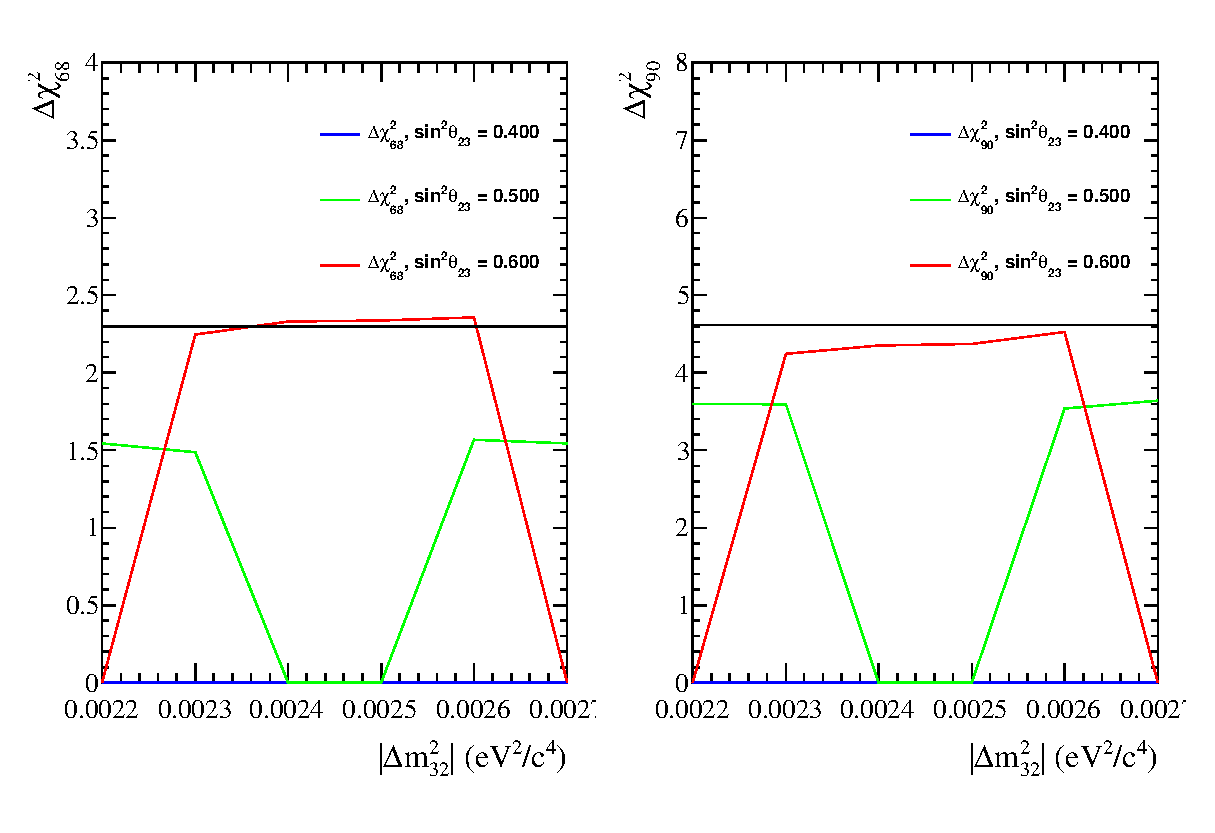
\includegraphics[width=30pc]{./images/fc_surface/FC_slice_dmsq}
\caption {
  Monte Carlo estimation,
  according to the method of Feldman and Cousins,
  of $\Delta\chi^{2}_{critical}$ values $\Delta\chi^{2}_{68}$ (left) and $\Delta\chi^{2}_{90}$ (right),
  as a function of $|\Delta{m^{2}_{32}}|$ for 3 different values of $\sin^{2}{\theta_{23}}$
  (0.40, 0.50 and 0.60).
  The $\Delta\chi^{2}_{critical}$ values were calculated
  from an ensemble of toy MC experiments, for an exposure of 6.3933$\times$10$^{20}$ POT,
  including both randomized systematic variations and statistical fluctuations.
  For comparison, the canonical value used in the constant-$\Delta\chi^{2}$
  method is also shown as a horizontal line.
  The normal mass hierarchy is assumed.
  It should be noted that the \emph{holes} in the surface are due to us being efficient with computing time.
}
\label{fig:fc_dchisqcrit_slice_dmsq:normal}
\end{figure*}


%...........................................................
%
% FC contours 
%

\begin{figure*}[htb]
\center
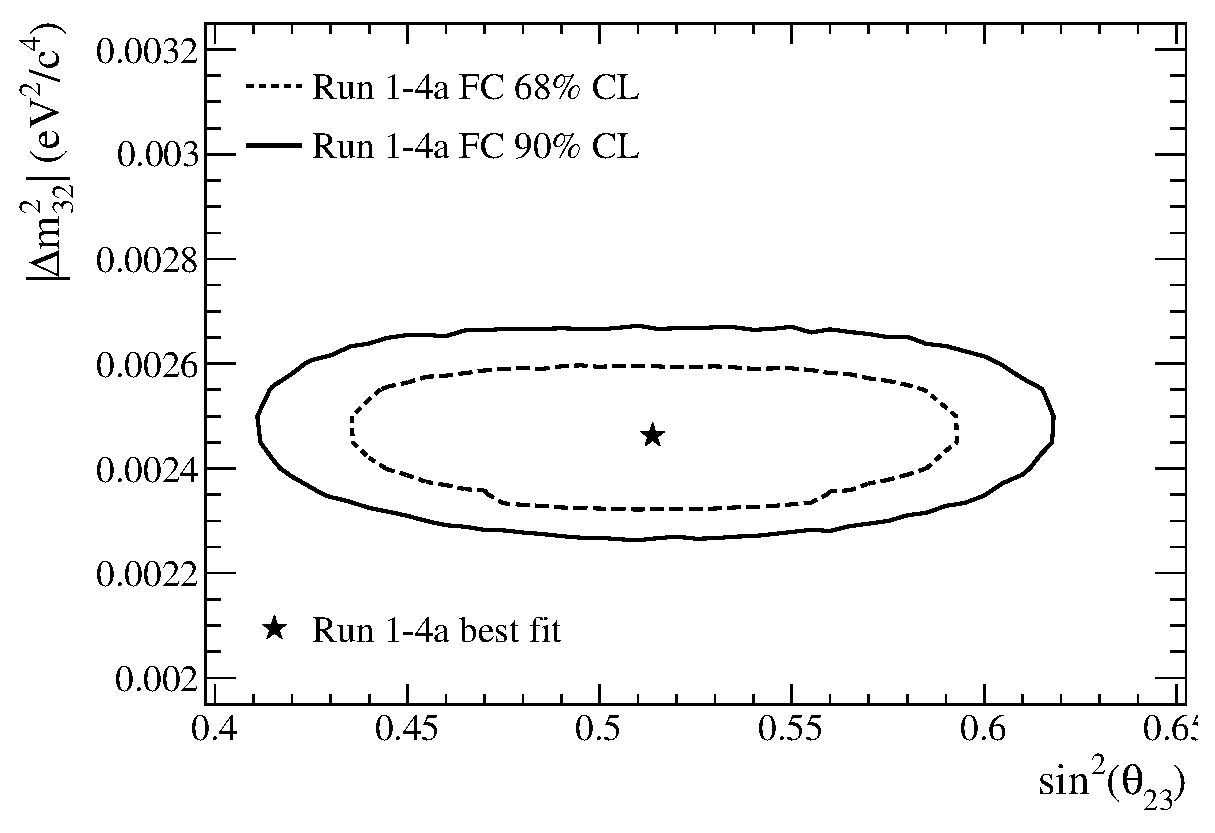
\includegraphics[width=35pc]{./images/data_results/run1234a_normal/contour_compare_normal_fconly}
\caption {
  68\% CL and 90\% CL allowed region (including systematics), 
  constructed with the method of Feldman and Cousins,
  for the fit to the Run 1+2+3+4a dataset.
  The best-fit point is also shown.
  The normal mass hierarchy is assumed.
  {\color{red}Smoother FC contours we be prepared for the final result.}
}
\label{fig:results_data1234a_fc_contour:normal}
\end{figure*}

% \begin{figure*}[htb]
% \center
% \includegraphics[width=35pc]{./images/data_results/run1234a_inverted/contour_compare_inverted_fconly}
% \caption {
%   68\% CL and 90\% CL allowed region (including systematics), 
%   constructed with the method of Feldman and Cousins,
%   for the fit to the Run 1+2+3+4a dataset.
%   The best-fit point is also shown.
%   The inverted mass hierarchy is assumed.
%  {\color{red}Smoother FC contours we be prepared for the final result.}
% }
% \label{fig:results_data1234a_fc_contour:inverted}
% \end{figure*}

\clearpage

%--------------------------------------------------------------------------------------
% Contour comparisons
%--------------------------------------------------------------------------------------

\subsection {Confidence region comparisons}
\label{sec:results_contour_comparisons}

The Run 1+2+3+4a 2-dimensional confidence regions obtained using the constant-$\Delta\chi^2$ method,
for the normal and inverted mass hierarchy assumptions,
are compared in Fig.\ \ref{fig:results_compare_normal_inverted:constdchisq}.
The effect of changing the mass hierarchy is large, and so it is important
that both contours be presented together.

The Run 1+2+3+4a 2-dimensional confidence regions obtained using the constant-$\Delta\chi^2$ and Feldman-Cousins methods
are compared in Figs.\ \ref{fig:results_compare_FC_constdchisq:normal} % and \ref{fig:results_compare_FC_constdchisq:inverted}
for the normal mass hierarchy assumption.
%and inverted mass hierarchy assumptions respectively.
The confidence regions produced
using the Feldman-Cousins method are narrower along $|\Delta{m^{2}_{32}}|$ at maximal disappearance than
those made with the constant-$\Delta\chi^{2}$ method.
The Feldman-Cousins contours are also wider
in $\sin^{2}{\theta_{23}}$ for values of $|\Delta{m^{2}_{32}}|$ near the best fit.

Comparisons were produced between our Run 1+2+3+4a result
MINOS (2013) \cite{MINOS2013sinsqtheta}, SuperK atmospherics 
(3-flavour 
zenith-angle analysis) (2012) \cite{SKAtm2012},
and T2K (Run 1+2+3) \cite{T2KRun123Disapp}.
The comparison is shown in Fig.\ \ref{fig:results_compare_FC_constdchisq_external}.
A second comparison with other results is shown in Fig.\ \ref{fig:results_compare_FC_constdchisq_external_sinsqtheta23},
between our Run 1+2+3+4a result
MINOS (2013) \cite{MINOS2013}, SuperK atmospherics 
(both the 2-flavour L/E and 3-flavour 
zenith-angle analyses) (2012) \cite{SKAtm2012},
and T2K (Run 1+2+3) \cite{T2KRun123Disapp}.
In this plot, the T2K Run 1+2+3+4a fit result has been converted from $\sin^2\theta_{23}$ to
$\sin^2(2\theta_{23})$ by profiling the octant.
This is the same method used by SuperK in their zenith angle contour, and,
if this method had been applied in the T2K Run 1+2+3 result, it should have
closely matched the T2K Run 1+2+3 $\theta_{23} \geq \pi/4$ contour.
T2K now has the world's best limit on $\theta_{23}$.

% In Fig.\ \ref{fig:results_compare_constdchisq_sensitivity}, 
% a comparison is shown
% between the Run 1+2+3+4a allowed region obtained 
% with constant-$\Delta\chi^{2}$ method, and the T2K 6.3933$\times$10$^{20}$ POT sensitivity
% contour produced at our best-fit point for the Run 1+2+3+4a dataset.
% The sensitivity contours were computed by averaging the contours of 1k toy-MC
% experiments generated with statistical fluctuations and all systematic parameters randomized.
% {\color{red} why not FC?}.

% Finally, a comparison between the confidence regions obtained by three 
% separate analyses of the Run 1+2+3+4a, Run 1+2+3 and Run 4a datasets 
% is shown in Fig.\ \ref{fig:results_compare_runs}.
% The contours from the different running periods are consistent.

%......................
%
% const Delta\chisq normal vs inverted
%
\begin{figure*}[htb]
\center
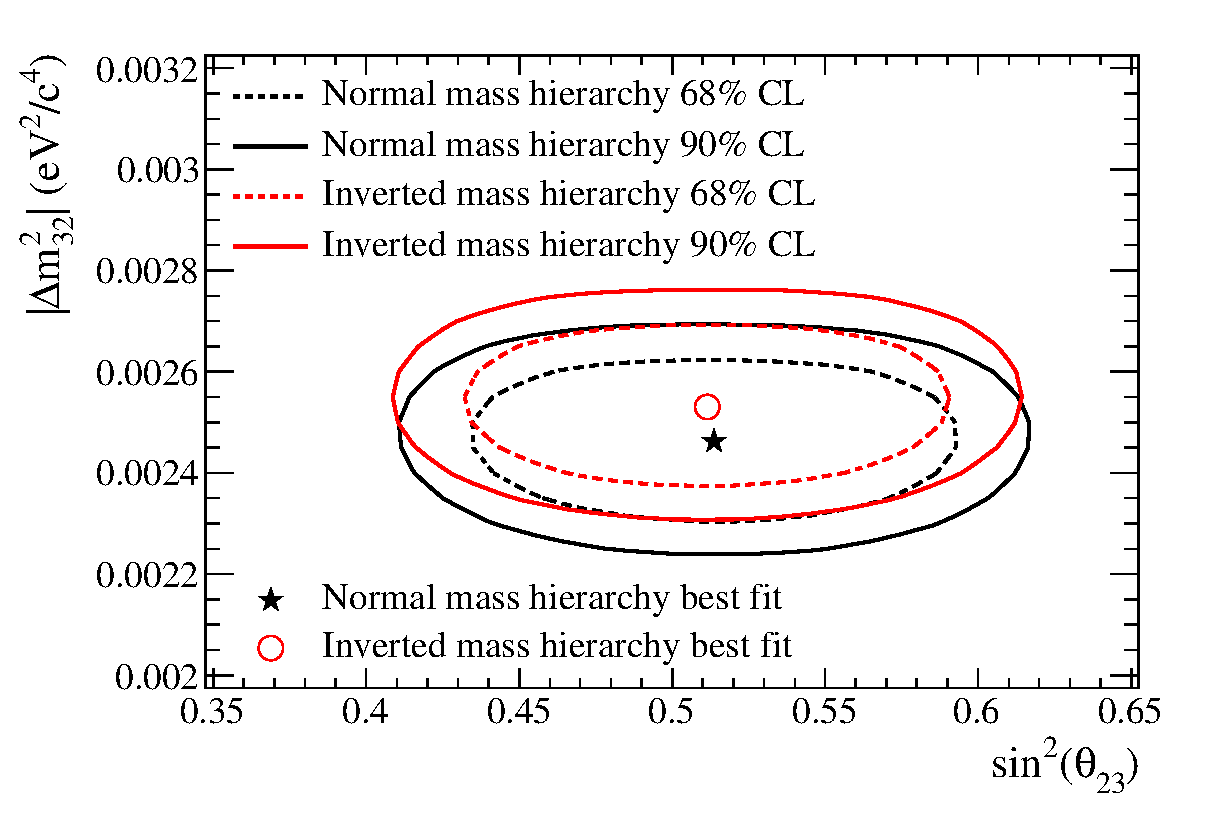
\includegraphics[width=30pc]{./images/data_results/compare/contours_run1-4a_nuis3fixdcp_hierarchies}
\caption {
  Comparison between the 68\% CL and 90\% CL allowed regions 
  obtained using the constant-$\Delta\chi^2$ method
  for the fit to the Run 1+2+3+4a dataset,
  for normal and inverted hierarchy assumptions.
}
\label{fig:results_compare_normal_inverted:constdchisq}
\end{figure*}

%......................
%
% const Delta\chisq vs FC (normal and inverted)
%
\begin{figure*}[htb]
\center
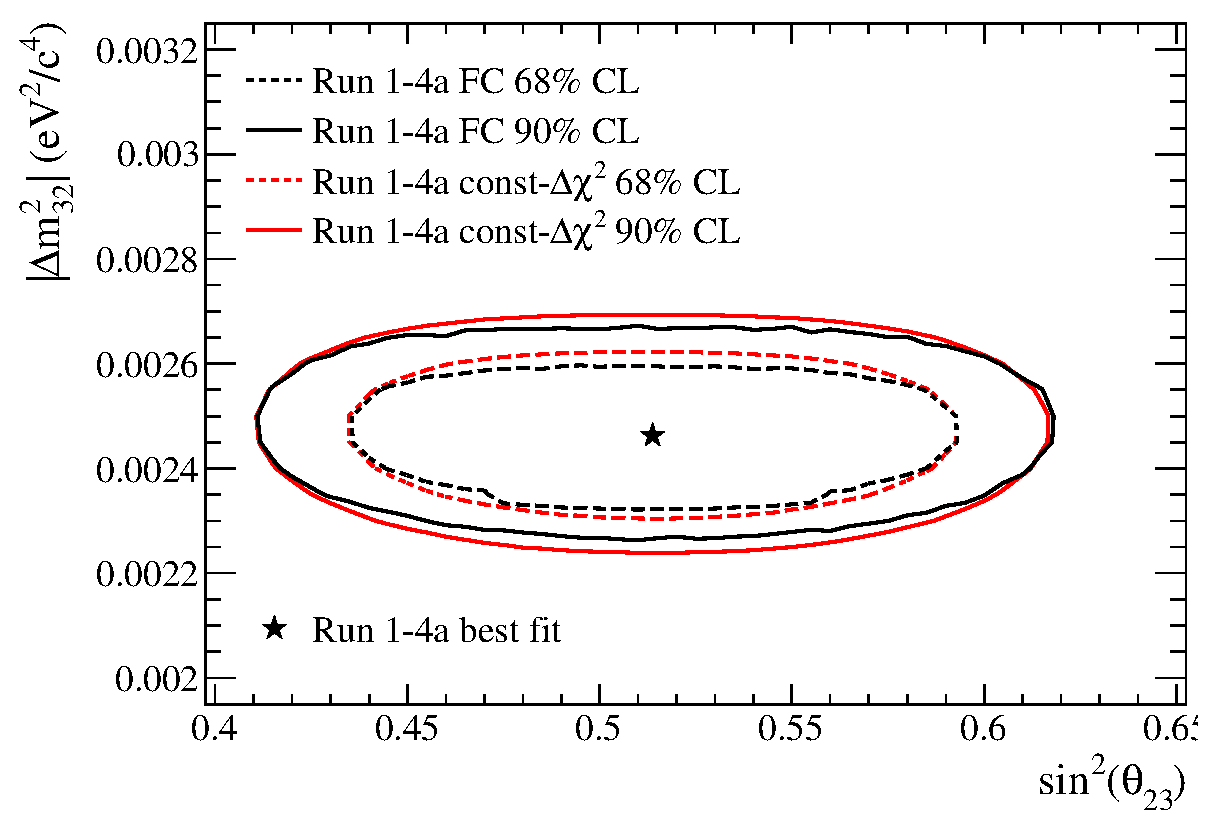
\includegraphics[width=30pc]{./images/data_results/run1234a_normal/contour_compare_normal_dcvsfc}
\caption {
  Comparison between the 68\% CL and 90\% CL allowed regions 
  obtained using the constant-$\Delta\chi^2$ and Feldman-Cousins methods 
  for the fit to the Run 1+2+3+4a dataset.
  The normal mass hierarchy is assumed.
  {\color{red}Smoother FC contours we be prepared for the final result.}
}
\label{fig:results_compare_FC_constdchisq:normal}
\end{figure*}

% \begin{figure*}[htb]
% \center
% 
\includegraphics[width=30pc]{./images/placeholder.eps}
% \caption {
%   Comparison between the 68\% CL and 90\% CL allowed regions 
%   obtained using the constant-$\Delta\chi^2$ and Feldman-Cousins methods 
%   for the fit to the Run 1+2+3+4a dataset.
%   The inverted mass hierarchy is assumed.
% }
% \label{fig:results_compare_FC_constdchisq:inverted}
% \end{figure*}


%......................
%
% VaLOR vs the world
%
\begin{figure*}[htb]
\center
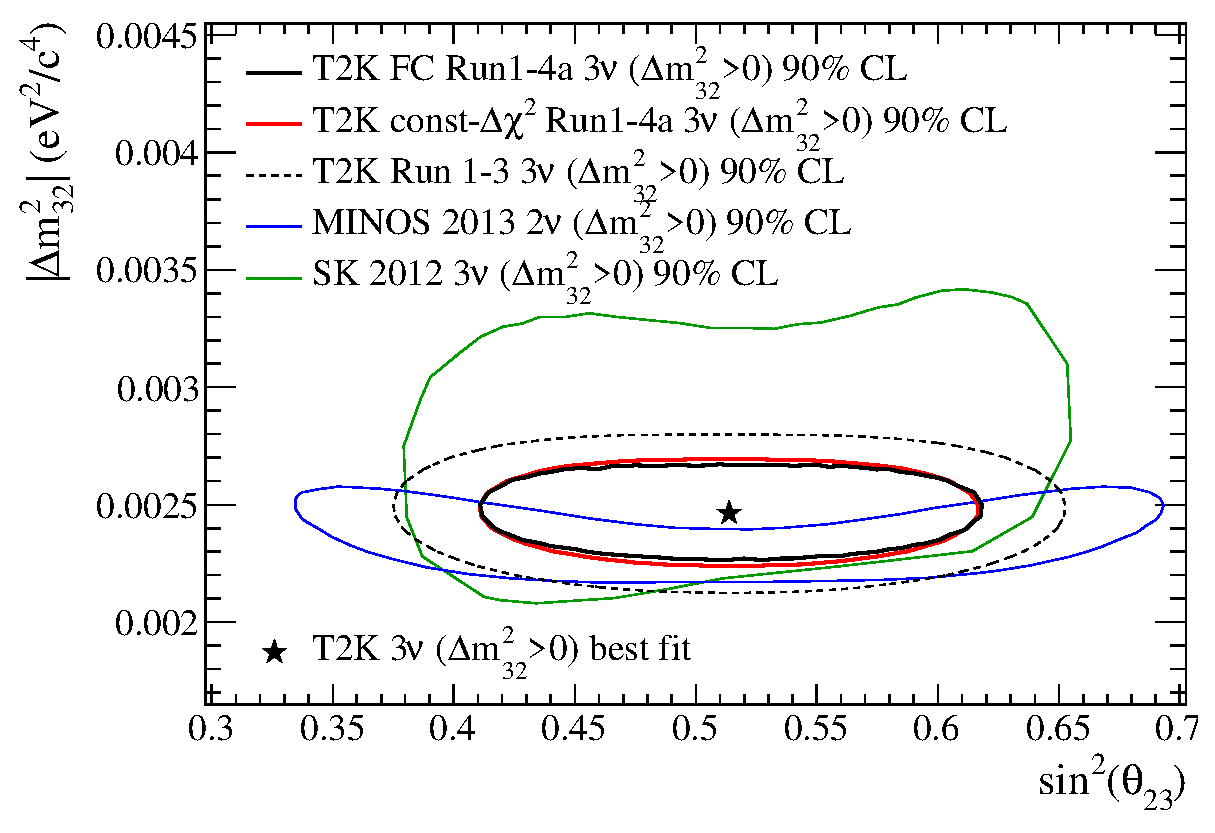
\includegraphics[width=30pc]{./images/data_results/compare/contour_compare_normal_dcvsfc_ext}
\caption {
  Comparison between 90\% CL allowed regions 
  from MINOS \cite{MINOS2013sinsqtheta}, SuperK atmospherics \cite{SKAtm2012}, T2K Run 1+2+3 \cite{T2KRun123Disapp},
  and the 90\% CL regions obtained from the VaLOR fit to the Run 1+2+3+4a dataset.
  Contours obtained using both the constant-$\Delta\chi^2$ and Feldman-Cousins methods are shown.
  The normal mass hierarchy is assumed for all results.
}
\label{fig:results_compare_FC_constdchisq_external}
\end{figure*}

\begin{figure*}[htb]
\center
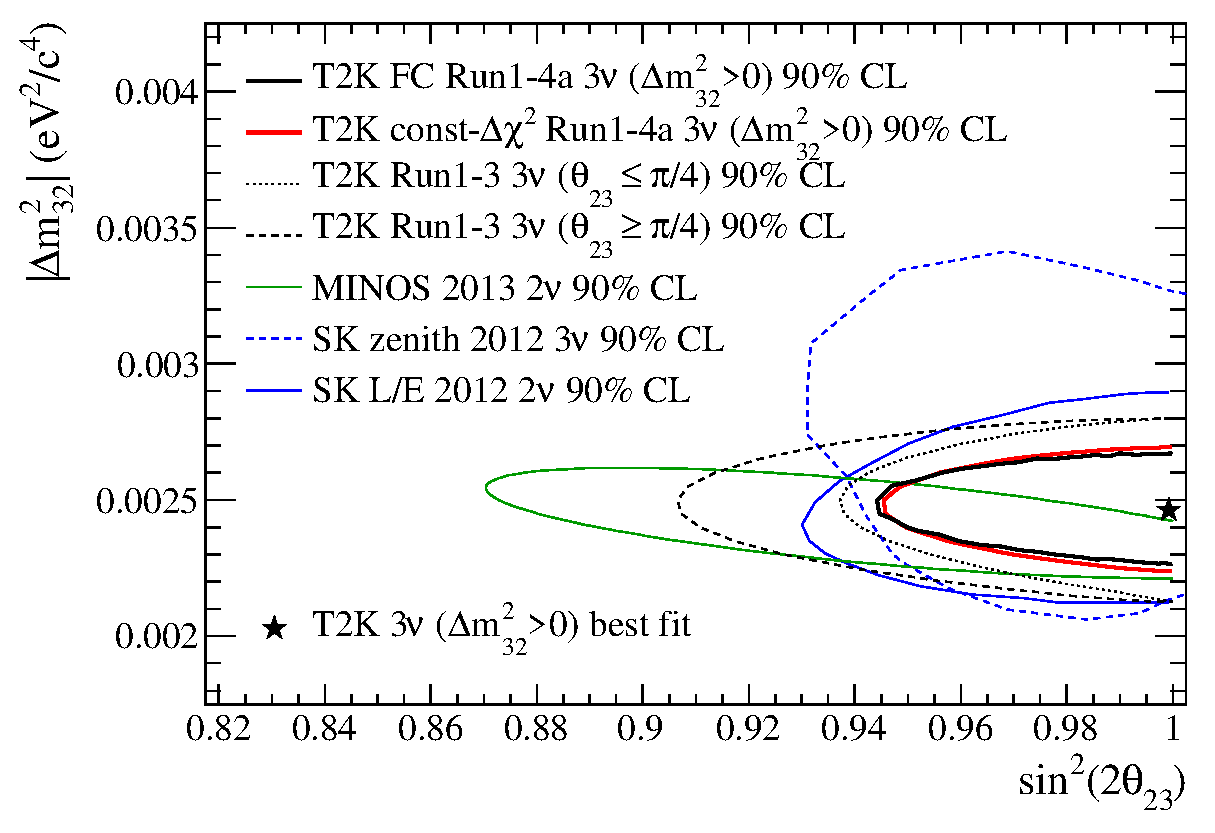
\includegraphics[width=30pc]{./images/data_results/compare/contour_compare_constdchisqfc_external_sinsq2theta23}
\caption {
  Comparison between 90\% CL allowed regions 
  from MINOS \cite{MINOS2013}, SuperK atmospherics \cite{SKAtm2012}, T2K Run 1+2+3 \cite{T2KRun123Disapp},
  and the 90\% CL regions obtained from the VaLOR fit to the Run 1+2+3+4a dataset.
  Contours obtained using both the constant-$\Delta\chi^2$ and Feldman-Cousins methods are shown.
  The normal mass hierarchy is assumed for all results.
}
\label{fig:results_compare_FC_constdchisq_external_sinsqtheta23}
\end{figure*}

%......................
%
% Comparison with sensitivity
%
% \begin{figure*}[htb]
% \center
% 
\includegraphics[width=30pc]{./images/placeholder.eps}
% \caption {
%   Comparison between the 68\% CL and 90\% CL allowed regions using the constant-$\Delta\chi^2$ 
%   method for the `2+8' fit to the Run 1+2+3 dataset
%   and the result of a sensitivity study at the `2+8' best-fit point for Run 1+2+3.
% }
% \label{fig:results_compare_28_constdchisq_sensitivity}
% \end{figure*}

%......................
%
% Run 1+2+3+4a vs Run 1+2+3 vs Run 4a
%
% \begin{figure*}[htb]
% \center
% 
\includegraphics[width=30pc]{./images/placeholder.eps}
% \caption {
%   Comparison between the 68\% CL and 90\% CL allowed regions obtained from separate
%   analyses to the Run 1+2+3+4a, Run 1+2+3 and Run 4a datasets.
%   All contours shown were calculated with the constant-$\Delta\chi^2$ method.
% }
% \label{fig:results_compare_runs}
% \end{figure*}


\clearpage

